\clearpage

\section {Results of the joint oscillation analysis with the Run 1+2+3 ($3.010 \times 10^{20}$ POT) dataset}
\label{sec:results}

\subsection {Best-fit oscillation parameters and systematic parameter pulls}
\label{sec:results_bestfit_params}

A joint 3-flavour oscillation fit, 
using the method described in Sec.\ \ref{sec:neutrino_oscillation_fitting}
was performed simultaneously on the 
single e-like ring and single $\mu$-like ring event reconstructed energy spectra
of the 3.010$\times$10$^{20}$ POT Run 1+2+3 dataset.
This fit allowed all 83 nuisance parameters considered in this work to float.
This analysis found
$|\Delta m^{2}|$ = 2.494 $\times$10$^{-3}$ $eV^{2}/c^{4}$,
$\sin^{2}\theta_{23}$ = 0.516,
$\sin^{2}\theta_{13}$ = 0.029 and
$\delta_{CP}$ = 2.086
to be the joint 3-flavour oscillation best-fit values for the Run 1+2+3 dataset for Normal Hierarchy
and 
$|\Delta m^{2}|$ =  2.468 $\times$10$^{-3}$ $eV^{2}/c^{4}$,
$\sin^{2}\theta_{23}$ = 0.516,
$\sin^{2}\theta_{13}$ = 0.034 and
$\delta_{CP}$ = 0.921
for Inverted Hierarchy.

Stand-alone 3-flavour $\nu_{\mu}$ disappearance and $\nu_{e}$ appearance analyses
were also performed on the Run 1+2+3 dataset.
In the stand-alone $\nu_{\mu}$ disappearance analysis,
$|\Delta m^{2}|$ and $\sin^{2}\theta_{23}$ were determined by fitting the 
single $\mu$-like ring event reconstructed energy spectrum
keeping $\sin^{2}\theta_{13}$ and $\delta_{CP}$ fixed, as was done in our published result,
and allowing all 57 nuisance parameters relevant to this analysis to float.
Similarly, in the stand-alone $\nu_{e}$ appearance analysis, 
$\sin^{2}\theta_{13}$ and $\delta_{CP}$ were determined by fitting the 
single e-like ring event reconstructed energy spectrum,
keeping $|\Delta m^{2}|$ and $\sin^{2}\theta_{23}$ fixed, as was done in our published result,
and allowing all 69 nuisance parameters relevant to this analysis to float.
The results of these fits are summarized in Tab.\ \ref{tab:data_fits:best_fit_values}. 
In this table are 
the relevant best-fit oscillation parameters, 
the observed and expected number of single e-like ring and single $\mu$-like ring events,
and goodness-of-fit figures.
Notice that the best-fit value for $\sin^{2}\theta_{23}$ is the same in both hierarchies 
although the best-fit value for the other parameters is different. The reason for this
result will be investigated in Sec. \ref{app:symmetry}.

The pull for each systematic parameter f included in the fit, is calculated as
\begin{equation}
\frac{f_{bf} - f_{nom}}{\sigma_{bf}},
\end{equation}
where 
$f_{bf}$ is the best-fit value of the systematic parameter,
$f_{nom}$ is the nominal value of the parameter (corresponding to no systematic variation), and
$\sigma_{bf}$ is the Migrad error output from Minuit.
The pulls of all systematic parameters allowed to float in the joint 3-flavour oscillation fit to the Run 1+2+3 dataset are shown in 
Figs.\ \ref{fig:run123_pulls_NH} for the fit assuming Normal Hierarchy, and in Fig.\ \ref{fig:run123_pulls_IH} for the fit assuming Inverted Hierarchy.
From these figures, it is apparent that most systematic parameters barely move from their nominal values.
We note that, although all relevant systematic parameters are allowed to float in these fits,
few of them move by more than $\pm$0.1$\sigma$. 
When a systematic parameter that is free to move stays close to its nominal value, this means that 
the reduction in $\chi^{2}$ from moving that parameter is less than the corresponding increase 
in the penalty term in equation \ref{eq:chisquare}. 
Only certain systematics are able to change the predicted reconstructed energy spectrum to a 
sufficient extent to offset the penalty term.

\subsection {Goodness-of-fit tests}
\label{sec:results_gof}

Goodness-of-fit tests were performed as described in Sec.\ \ref{sec:goodness_of_fit},
and the p-values for the joint 3-flavour oscillation fit and
the stand-alone $\nu_{\mu}$ disappearance and $\nu_{e}$ appearance fits to the Run 1+2+3 dataset
are shown in Tab.\ \ref{tab:data_fits:best_fit_values}. 
The $\chi^2$ distributions from which the p-values were calculated are shown for the 
Run 1+2+3 joint 3-flavour oscillation fit in Fig.\ \ref{fig:run123_gofchisq} (\ref{fig:run123_gofchisq_ih}),
while for the stand-alone $\nu_{\mu}$ disappearance fit it is shown in Fig.\ \ref{fig:run123_gofchisq_disapp} (\ref{fig:run123_gofchisq_disapp_ih}) 
and for the stand-alone $\nu_{e}$ appearance it is shown in Fig.\ \ref{fig:run123_gofchisq_app} ( \ref{fig:run123_gofchisq_app_ih})
for Normal (Inverted) Hierarchy. All fits have a high degree of plausibility.


%...........................................................
%
% Table summarizing best-fit results
%
\begin{table}[htb]
\scriptsize
\centering
\begin{tabular}{| l | l | l | c  c  c  c | c  c  c  c | c  c |}
\hline
Analysis & Run & Hierarchy/ &
$|\Delta m^{2}|$ & sin$^2\theta_{23}$ & sin$^2\theta_{13}$ & $\delta_{CP}$ & 
N$_{obs}^{1R\mu}$ & N$_{exp}^{1R\mu}$ & 
N$_{obs}^{1Re}$ & N$_{exp}^{1Re}$ & 
$\chi^2/ndf$ & p-value \\
 &  & Octant & $10^{-3} eV^{2}/c^{4}$ & & & & & & & & & \\
\hline
2012 joint              & 1+2+3 & NH/1st & 2.494 & 0.516 & 0.029 & 2.086 &    58 & 57.697 & 11 & 10.452 & 72.26/94 & 0.86 \\
2012 $\nu_{\mu}$ disap. & 1+2+3 & NH/1st & 2.479 & 0.514 & --    & --    &    58 & 57.901 & 11 & --    & 56.05/71 & 0.90 \\
2012 $\nu_{e}$ app.     & 1+2+3 & NH/1st & --    & --    & 0.023 & 0(fixed) &    58 & --    & 11 & 10.477 & 16.47/24 & 0.67 \\
\hline
2012 joint              & 1+2+3 & NH/2nd & 2.493 & 0.516 & 0.029 & 2.074 &      58 & 57.712 & 11 & 10.452 & 72.26/94 &  \\
2012 $\nu_{\mu}$ disap. & 1+2+3 & NH/2nd & 2.479 & 0.514 & --    & --    &     58 & 57.903 & 11 & --    & 56.05/71 &  \\
2012 $\nu_{e}$ app.     & 1+2+3 & NH/2nd & --    & --    & 0.023 & 0(fixed) &     58 & --    & 11 & 10.477 & 16.47/24 &  \\
\hline
2012 joint              & 1+2+3 & IH/1st & 2.468 & 0.516 & 0.034 & 0.921 &      58 & 57.715 & 11 & 10.454 & 72.26/94 & 0.85 \\
2012 $\nu_{\mu}$ disap. & 1+2+3 & IH/1st & 2.474 & 0.512 & --    & --    &      58 & 57.891 & 11 & --    & 56.05/71 & 0.90 \\
2012 $\nu_{e}$ app.     & 1+2+3 & IH/1st & --    & --    & 0.029 & 0(fixed) &     58 & --    & 11 & 10.435 & 16.42/24 & 0.58 \\
\hline
2012 joint              & 1+2+3 & IH/2nd & 2.468 & 0.516 & 0.034 & 0.922 &      58 & 57.723 & 11 & 10.454 & 72.26/94 &  \\
2012 $\nu_{\mu}$ disap. & 1+2+3 & IH/2nd & 2.474 & 0.512 & --    & --    &    58 & 57.891 & 11 & --    & 56.05/71 &  \\
2012 $\nu_{e}$ app.     & 1+2+3 & IH/2nd & --    & --    & 0.029 & 0(fixed) &     58 & --    & 11 & 10.435 & 16.42/24 &  \\
\hline
\end{tabular}
\caption{
  Summary of best-fit parameters for the joint 3-flavour oscillation fit,
  and the stand-alone 3-flavour $\nu_{\mu}$ disappearance and $\nu_{e}$ appearance fits
  to the Run 1+2+3 dataset.
  The quoted best-fit $\chi^2$ values were computed from the test-statistic minimized in the fit (likelihood ratio)
  with the reconstructed energy binning used in each fit.
  The table also shows the p-values obtained from the goodness-of-fit test of Sec.\ \ref{sec:goodness_of_fit}.
}
\label{tab:data_fits:best_fit_values}
\end{table}

%
% Spectra
%

\subsection {Best-fit single e-like ring and single $\mu$-like ring event reconstructed energy spectra}
\label{sec:results_bestfit_spectra}

The reconstructed neutrino energy distribution of single $\mu$-like ring (single e-like ring) events 
in the Run 1+2+3 dataset is shown in Fig.\ \ref{fig:run123_1Rmu_bestfit_spectrum_nh} (Fig.\ \ref{fig:run123_1Re_bestfit_spectrum_nh})
along with best-fit prediction of the joint 3-flavour oscillation analysis, assuming Normal Hierarchy.
In Fig.\ \ref{fig:run123_1Rmu_bestfit_spectrum_nh}
we superimpose the best-fit prediction from the stand-alone 3-flavour $\nu_{\mu}$ disappearance analysis,
while in In Fig.\ \ref{fig:run123_1Re_bestfit_spectrum_nh}
we superimpose the best-fit prediction from the stand-alone 3-flavour $\nu_{e}$ appearance analysis.
The distributions are shown with the reconstructed neutrino energy binning
that was used in the fitting procedure (see footnote 2 in Sec.\ \ref{sec:prediction}).
The single $\mu$-like ring (single e-like ring) 
best-fit prediction of the joint 3-flavour oscillation analysis, assuming Inverted Hierarchy,
are shown in Fig.\ \ref{fig:run123_1Rmu_bestfit_spectrum_ih} (Fig.\ \ref{fig:run123_1Re_bestfit_spectrum_ih}).

Since the reconstructed energy binning used in the fit is relatively fine, 
it can be beneficial to see the above distributions using a coarser binning scheme\footnote{
  For the single $\mu$-like ring event sample
  16 reconstructed energy bins are used arranged as follows:
  1 0.3-GeV bin in 0 - 0.3 GeV,
  8 0.1-GeV bins in 0.3 - 1.1 GeV,
  1 0.15-GeV bin in 1.1 GeV - 1.25 GeV,
  1 0.25-GeV bin in 1.25 - 1.5 GeV GeV,
  1 0.5-GeV bin in 1.5 - 2 GeV,
  2 1-GeV bin in 2-4 GeV,
  1 2-GeV bin in 4-6 GeV and 1 bin above 6 GeV.
  For the single e-like ring event sample 4 0.3 GeV bins in 0-1.2 GeV are used.
}. 
The re-binned reconstructed neutrino energy distribution of single $\mu$-like ring and single e-like ring events for both mass hierarchies
are shown in Figs.\ \ref{fig:run123_1Rmu_bestfit_spectrum_nh_coarse} - \ref{fig:run123_1Re_bestfit_spectrum_ih_coarse}.

Finally, the ratio of the best-fit reconstructed neutrino energy distribution of single $\mu$-like ring (single e-like ring)
events obtained from the joint 3-flavour oscillation analysis and the stand-alone  $\nu_{\mu}$ disappearance ( $\nu_{e}$ appearance) analysis
is shown in Fig.\ \ref{fig:run123_1Rmu_bestfit_spectrum_ratio_nh} (Fig.\ \ref{fig:run123_1Re_bestfit_spectrum_ratio_nh}) for Normal Hierarchy and
in Fig.\ \ref{fig:run123_1Rmu_bestfit_spectrum_ratio_ih} (Fig.\ \ref{fig:run123_1Re_bestfit_spectrum_ratio_ih}) for Inverted Hierarchy.

The best-fit single $\mu$-like ring reconstructed energy spectrum from the joint analysis is almost identical to that from the stand-alone $\nu_{\mu}$-disappearance analysis from 0.6 - 1.2 GeV, 
but is slightly lower from 0.3 - 0.6 GeV and $>$1.2 GeV, and this is true for both mass hierarchies. 
Meanwhile the ratio of the best-fit single e-like ring reconstructed energy spectrum from the joint analysis to that from the stand-alone $\nu_{e}$-appearance analysis 
shows different behaviour for the two hierarchies. For the normal hierarchy (NH), this ratio is $<$1 from 0.1 - 0.3 GeV, $>$1 from 0.3 - 0.55 GeV, and $<$1 above 0.55 GeV. 
However, for the inverted hierarchy (IH) the ratio is $<$1 from 0.1 - 0.6 GeV and $>$1 above 0.6 GeV. 

%
% Contours
%

\subsection {Confidence regions}
\label{sec:results_confidence_regions}

The marginalized $\Delta\chi^2$ distribution as function
of each of $|\Delta m^{2}|$, $sin^{2}\theta_{23}$, $sin^{2}\theta_{13}$ and $\delta_{CP}$
oscillation parameters for the joint 3-flavour oscillation fit to the Run 1+2+3 dataset 
is shown in Figs.\ \ref{fig:run123_dchisq_Dmsq_nh} - \ref{fig:run123_dchisq_deltacp_nh}.
From these plots,
the 90\% (68\%) CL allowed region for the four oscillation parameters can be summarized as
2.227$\times$10$^{-3}$ (2.332$\times$10$^{-3}$) $eV^{2}/c^{4}$
$< |\Delta m^{2}| < $
2.773$\times$10$^{-3}$ (2.659$\times$10$^{-3}$) $eV^{2}/c^{4}$,
0.401 (0.433) $< sin^{2}\theta_{23} <$ 0.628 (0.596),
0.006 (0.012) $< sin^{2}\theta_{13} <$ 0.058 (0.048) and
-$\pi$ (-$\pi$) $< \delta_{CP} <$ $\pi$ ($\pi$)
for Normal Hierarchy and
2.218 $\times$10$^{-3}$ (2.311$\times$10$^{-3}$) $eV^{2}/c^{4}$
$< |\Delta m^{2}| < $
2.729 $\times$10$^{-3}$ (2.627$\times$10$^{-3}$) $eV^{2}/c^{4}$,
 0.397 (0.433) $< sin^{2}\theta_{23} <$ 0.627 (0.596),
0.006 (0.013) $< sin^{2}\theta_{13} <$ 0.069 (0.054) and
-$\pi$ (-$\pi$) $< \delta_{CP} <$ $\pi$ ($\pi$)
for Inverted Hierarchy.

The correlations between the oscillation parameters were also studied.
In Figs.\ \ref{fig:run123_confreg_sinsqtheta23_Dmsq_nh} - \ref{fig:run123_confreg_sinsqtheta23_sinsqtheta13_nh}, 
we present, respectively, the 
the 68\% and 90\% CL regions in the following four 2-dimensional oscillation parameter spaces:
($sin^{2}\theta_{23}$, $|\Delta m^{2}|$),
($sin^{2}\theta_{13}$, $|\Delta m^{2}|$),
($sin^{2}\theta_{13}$, $\delta_{CP}$) and
($sin^{2}\theta_{23}$, $sin^{2}\theta_{13}$).
Results from the stand-alone Run 1+2+3 $\nu_{\mu}$ disappearance and $\nu_{e}$ appearance 
analyses are superimposed wherever possible.

Comparisons between the confidence regions obtain from the joint 3-flavour oscillation fits
under difference mass hierarchy assumptions are shown in Figs.\ \ref{fig:run123_dchisq_Dmsq_hcomp} - \ref{fig:run123_confreg_sinsqtheta23_sinsqtheta13_hcomp}.
%Comparisons between the confidence regions obtain from the joint 3-flavour oscillation fits, for the Normal Hierarchy,
%but using initial fit values in the different octants are shown in Figs.\ \ref{fig:run123_dchisq_Dmsq_octcomp} - \ref{fig:run123_confreg_sinsqtheta13_Dmsq_octcomp}.

To construct the plots shown in this subsection, the same procedure is followed 
as in Appendix \ref{app:fake_dataset_fits}.
In joint 3-flavour analysis plots,
the value of $\chi^2$ was minimized with respect to all 83 nuisance parameters
and the oscillation parameters not shown on the plot (except from the solar parameters,
$sin^{2}\theta_{12}$ and $\delta m^{2}$ which, as shown in Appendix \ref{app:solar}, 
have a negligible effect and they are fixed to constant values for all the joint and stand-alone analyses).
In the plots shown for the stand-alone $\nu_{\mu}$ disappearance analysis, unless explicitly stated,
$sin^{2}\theta_{13}$ and $\delta_{CP}$ are fixed to constant values,
as was done for our published results,
and $\chi^2$ was minimized with respect to all 48 nuisance parameters
relevant to that analysis.
Similarly, for the stand-alone $\nu_{e}$ appearance analysis, unless explicitly stated,
$sin^{2}\theta_{23}$ and $|\Delta m^{2}|$ are also fixed to constant values,
as was done for our published results,
and $\chi^2$ was minimized with respect to all 64 nuisance parameters
relevant to that analysis.

The $\Delta \chi^{2}$ distributions of $|\Delta m^{2}|$ and $\sin^{2}\theta_{23}$ are almost identical for the joint analysis and the stand-alone $\nu_{\mu}$-disappearance analysis. 
However the $\Delta \chi^{2}$ distribution of $\sin^{2}\theta_{13}$ is wider for the joint analysis than for the stand-alone $\nu_{e}$-appearance analysis. 
This is due to the partial degeneracy of this parameter with $\sin^{2}\theta_{23}$ when fitting the single e-like ring sample. Since $\sin^{2}\theta_{23}$ 
is fitted in the joint analysis, the $\Delta \chi^{2}$ distribution of $\sin^{2}\theta_{13}$ is wider than in the stand-alone analysis in which $\sin^{2}\theta_{23}$ is fixed. 
There is very good agreement between the confidence contours in the ($\sin^{2}\theta_{23}$, $|\Delta m^{2}|$) space from the joint analysis and those from the 
stand-alone $\nu_{\mu}$-disappearance analysis. Contours in the ($\sin^{2}\theta_{13}$, $\delta_{CP}$) space are wider for the joint analysis with respect to the contours
obtained for the stand-alone appearance analysis. The main reason is the different method used (global minimum vs raster scan). In Figs. \ref{fig:run123_confreg_sinsqtheta13_deltacp_raster_nh}
and \ref{fig:run123_confreg_sinsqtheta13_deltacp_raster_ih} the same method (raster scan) was used for both the joint and the stand-alone appearance analysis to fit
Run1+2+3 dataset in Normal and Inverted Hierarchy respectively. Contours from the joint analysis agree very well with those from the 
stand-alone $\nu_{e}$-appearance analysis when using the raster scan method in both analyses. 

The $\Delta \chi^{2}$ distributions for $|\Delta m^{2}|$ and $\sin^{2}\theta_{23}$  are very similar between the NH and IH. However the distribution for $\sin^{2}\theta_{13}$ 
and $\delta_{CP}$ is shifted to higher values for the IH compared with the NH, while the distribution for $\delta_{CP}$ is shifted to lower values. 
The confidence contours in the ($\sin^{2}\theta_{23}$, $|\Delta m^{2}|$) space agree very well between the NH and IH, but the upper 
limit in the ($\sin^{2}\theta_{13}$, $\delta_{CP}$) space is higher for the IH than for the NH.

%All the $\Delta \chi^{2}$ distributions and confidence regions agree very well between the initial value of $\sin^{2}\theta_{23}$ being in the first octant and in the second octant.


%...........................................................
%
% pulls
%

\begin{figure*}[htb]
\center
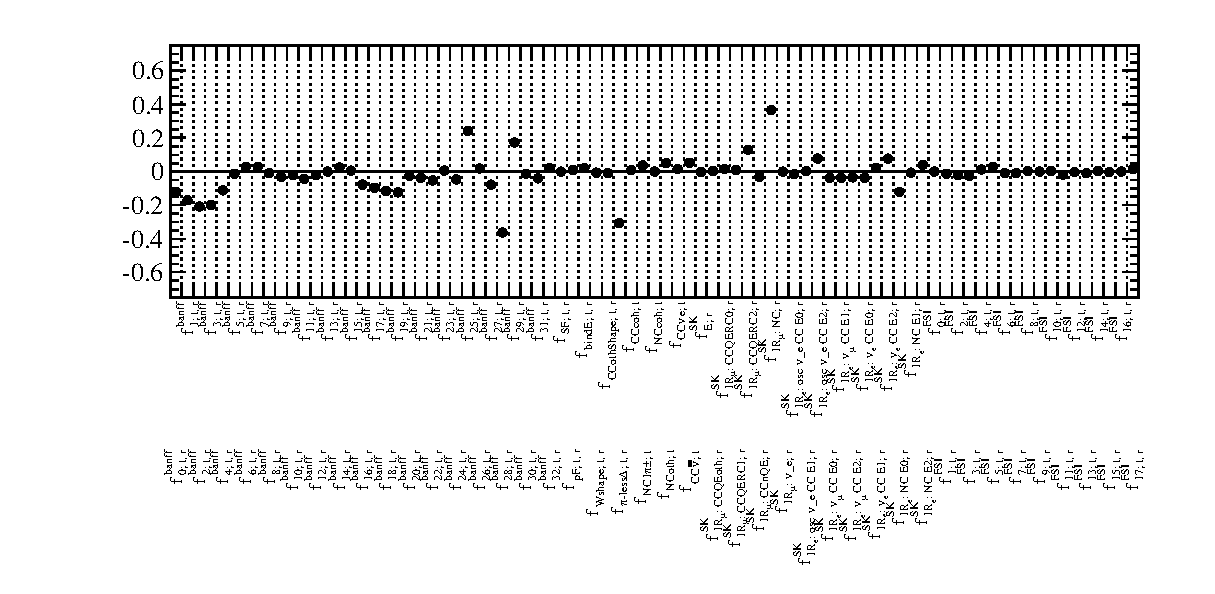
\includegraphics[width=55pc,angle=270]{./images/results/pulls_data_nh_1st.eps}
\caption {
  Systematic parameter pulls for the 83 systematics allowed to float 
  in the Run 1+2+3 joint 3-flavour oscillation fit with Normal Hierarchy.
}
\label{fig:run123_pulls_NH}
\end{figure*}

\begin{figure*}[htb]
\center
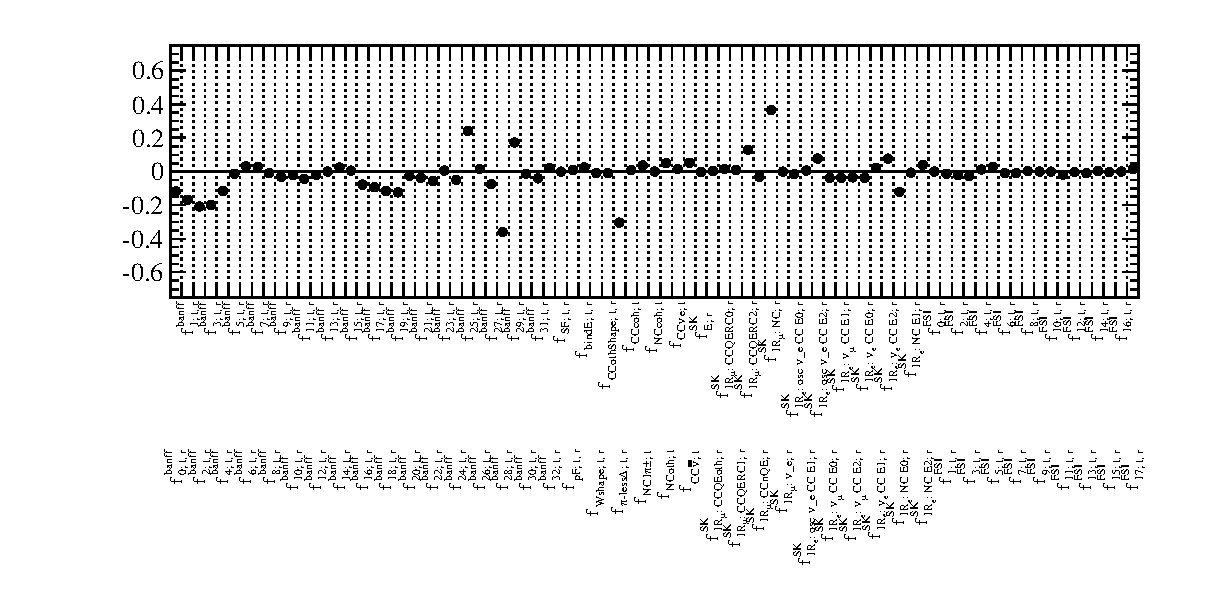
\includegraphics[width=55pc,angle=270]{./images/results/pulls_data_ih_1st.eps}
\caption {
  Systematic parameter pulls for the 83 systematics allowed to float 
  in the Run 1+2+3 joint 3-flavour oscillation fit with Inverted Hierarchy.
}
\label{fig:run123_pulls_IH}
\end{figure*}




%...........................................................
%
% chisq distributions used for calculating the fit p-values
%

\begin{figure*}[htb]

\begin{minipage}[t]{0.90\linewidth}
\center
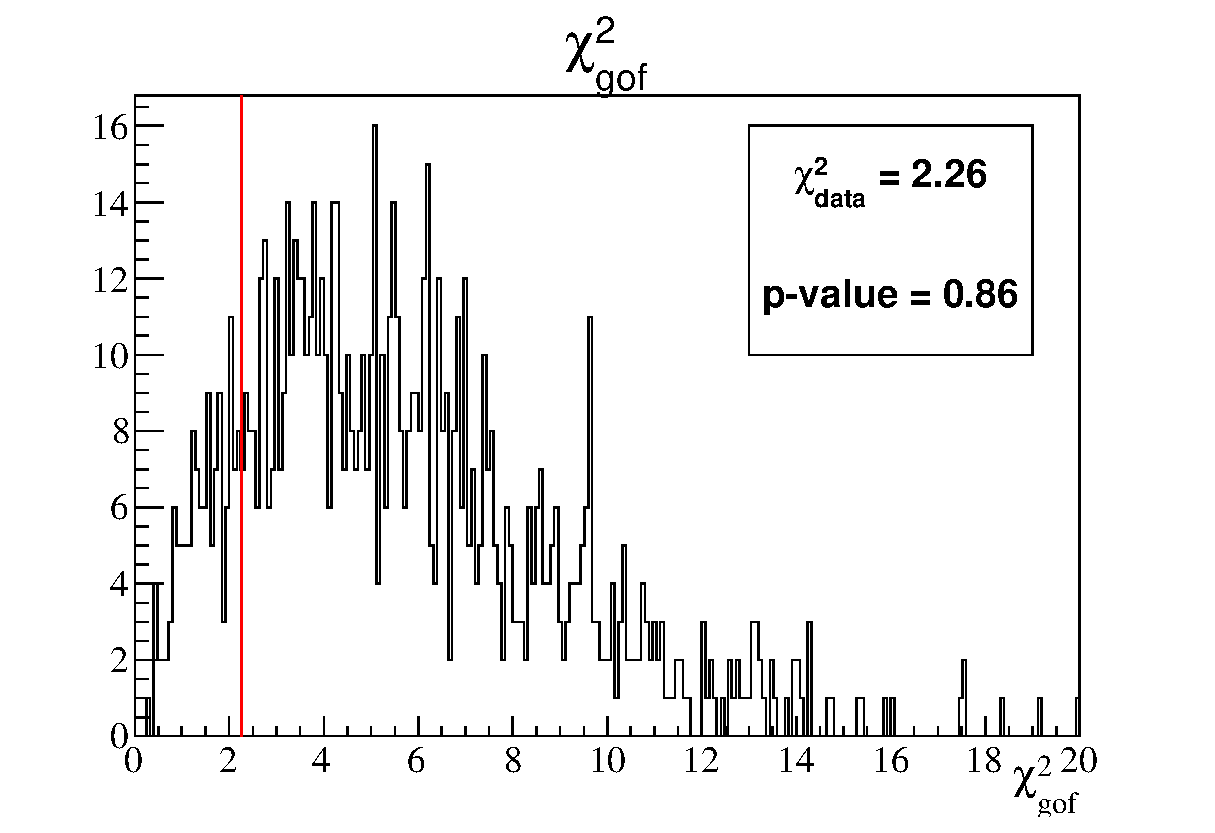
\includegraphics[width=30pc]{./images/results/data_nh_1st_gof_new.eps}
\caption {
  Distribution of $\chi^2_{gof}$, the goodness-of-fit (gof) $\chi^2$, 
  from 1k toy MC experiments generated at the Run 1+2+3 joint 3-flavour analysis best-fit oscillation point
  with Normal Hierarchy.
  The $\chi^2_{gof}$ value for the Run 1+2+3 data ($\chi^2_{data}$) is highlighted.
  All $\chi^2_{gof}$ values were computed 
  using the 5 (single $\mu$-like ring) + 3 (single e-like ring) 
  reconstructed energy binning scheme described in Sec.\ \ref{sec:goodness_of_fit},
}
\label{fig:run123_gofchisq}
\end{minipage}

\vfill
\vspace*{0.7cm}

\begin{minipage}[t]{0.46\linewidth}
\center
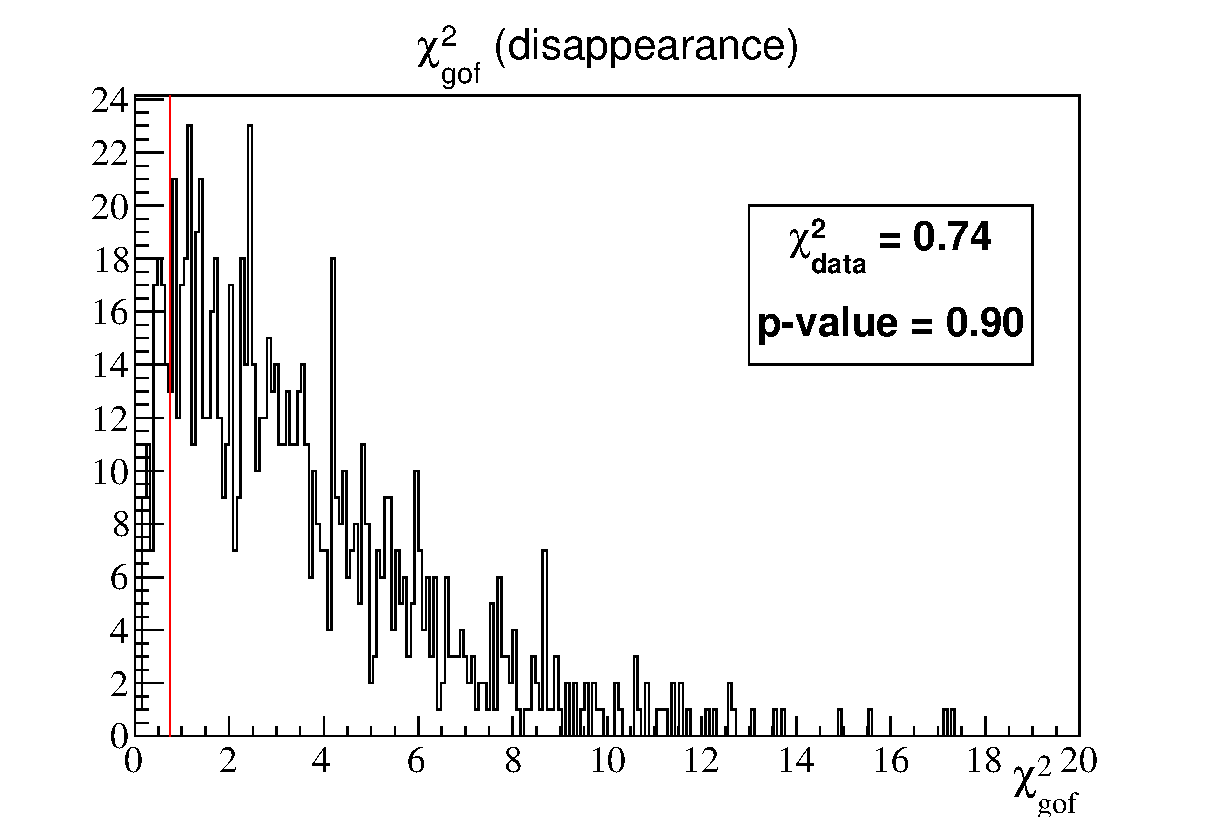
\includegraphics[width=18pc]{./images/results/data_nh_1st_gof_disap_new.eps}
\caption {
  Distribution of $\chi^2_{gof}$
  from 1k toy MC experiments generated at the Run 1+2+3 stand-alone 3-flavour $\nu_{\mu}$ disappearance analysis 
  best-fit oscillation point with Normal Hierarchy.
  The $\chi^2_{gof}$ value for the Run 1+2+3 data ($\chi^2_{data}$) is highlighted.
  All $\chi^2_{gof}$ values were computed 
  using the 5 (single $\mu$-like ring) 
  reconstructed energy binning scheme described in Sec.\ \ref{sec:goodness_of_fit},
}
\label{fig:run123_gofchisq_disapp}
\end{minipage}
\hspace{0.03\linewidth}
\begin{minipage}[t]{0.46\linewidth}
\center
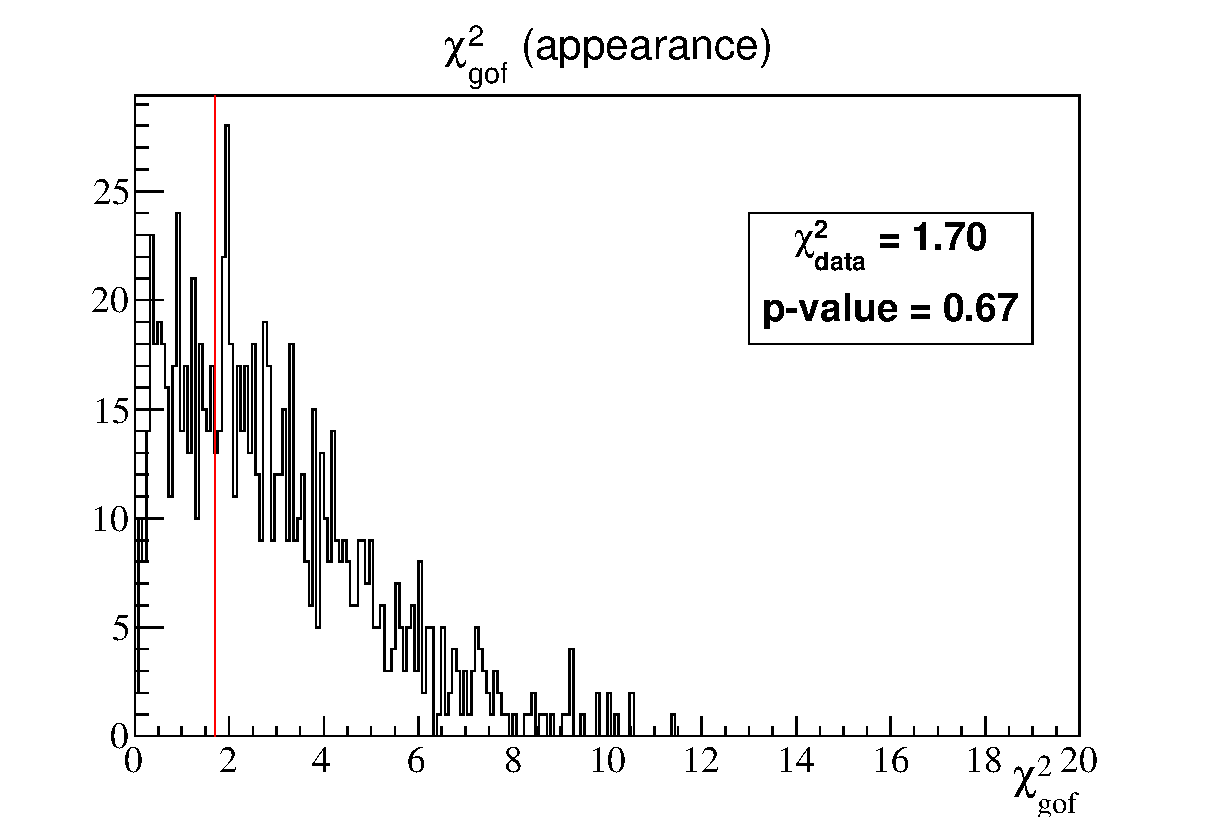
\includegraphics[width=18pc]{./images/results/data_nh_1st_gof_app_new.eps}
\caption {
  Distribution of $\chi^2_{gof}$
  from 1k toy MC experiments generated at the Run 1+2+3 stand-alone 3-flavour $\nu_{e}$ appearance analysis 
  best-fit oscillation point with Normal Hierarchy.
  The $\chi^2_{gof}$ value for the Run 1+2+3 data ($\chi^2_{data}$) is highlighted.
  All $\chi^2_{gof}$ values were computed 
  using the 3 (single e-like ring) 
  reconstructed energy binning scheme  as described in Sec.\ \ref{sec:goodness_of_fit},
}
\label{fig:run123_gofchisq_app}
\end{minipage}

\end{figure*}


\begin{figure*}[htb]

\begin{minipage}[t]{0.90\linewidth}
\center
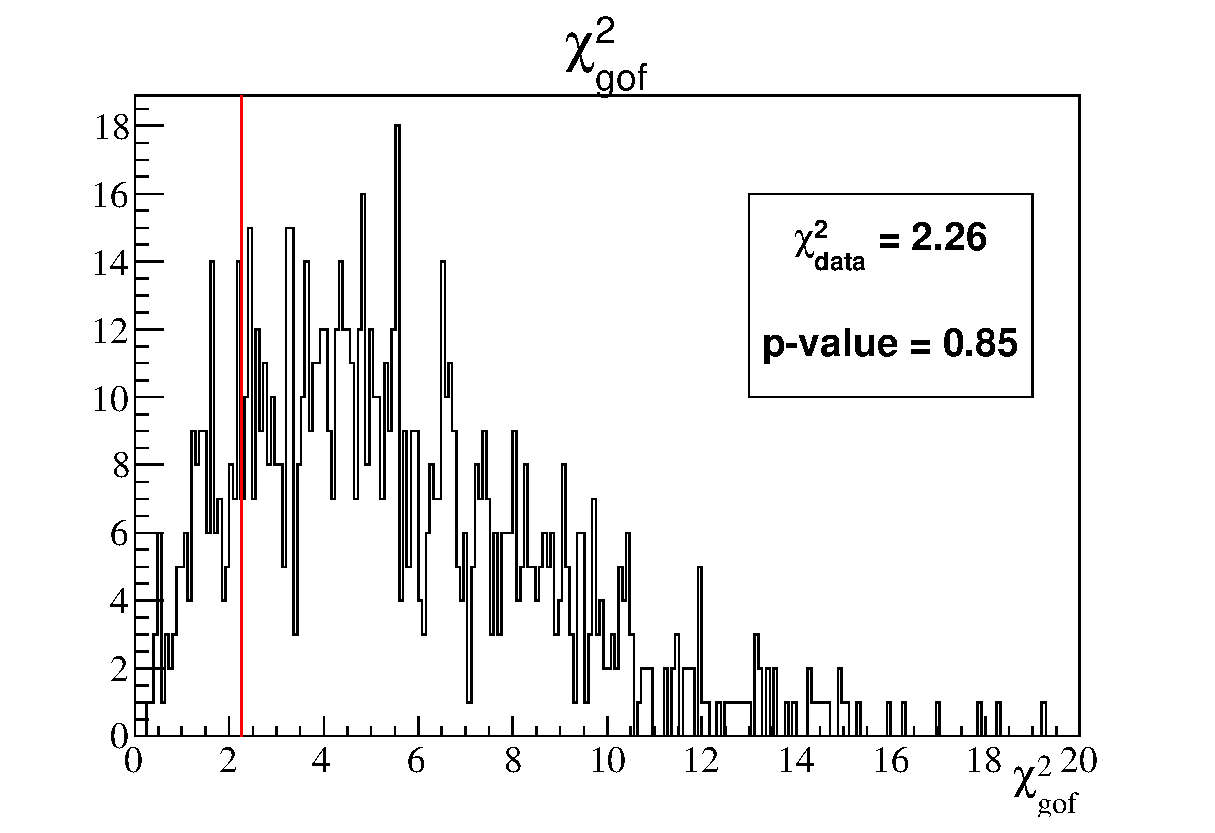
\includegraphics[width=30pc]{./images/results/data_ih_1st_gof_new.eps}
\caption {
  Distribution of $\chi^2_{gof}$, the goodness-of-fit (gof) $\chi^2$, 
  from 1k toy MC experiments generated at the Run 1+2+3 joint 3-flavour analysis best-fit oscillation point
  with Inverted Hierarchy.
  The $\chi^2_{gof}$ value for the Run 1+2+3 data ($\chi^2_{data}$) is highlighted.
  All $\chi^2_{gof}$ values were computed 
  using the 5 (single $\mu$-like ring) + 3 (single e-like ring) 
  reconstructed energy binning scheme described in Sec.\ \ref{sec:goodness_of_fit}.
}
\label{fig:run123_gofchisq_ih}
\end{minipage}

\vfill
\vspace*{0.7cm}

\begin{minipage}[t]{0.46\linewidth}
\center
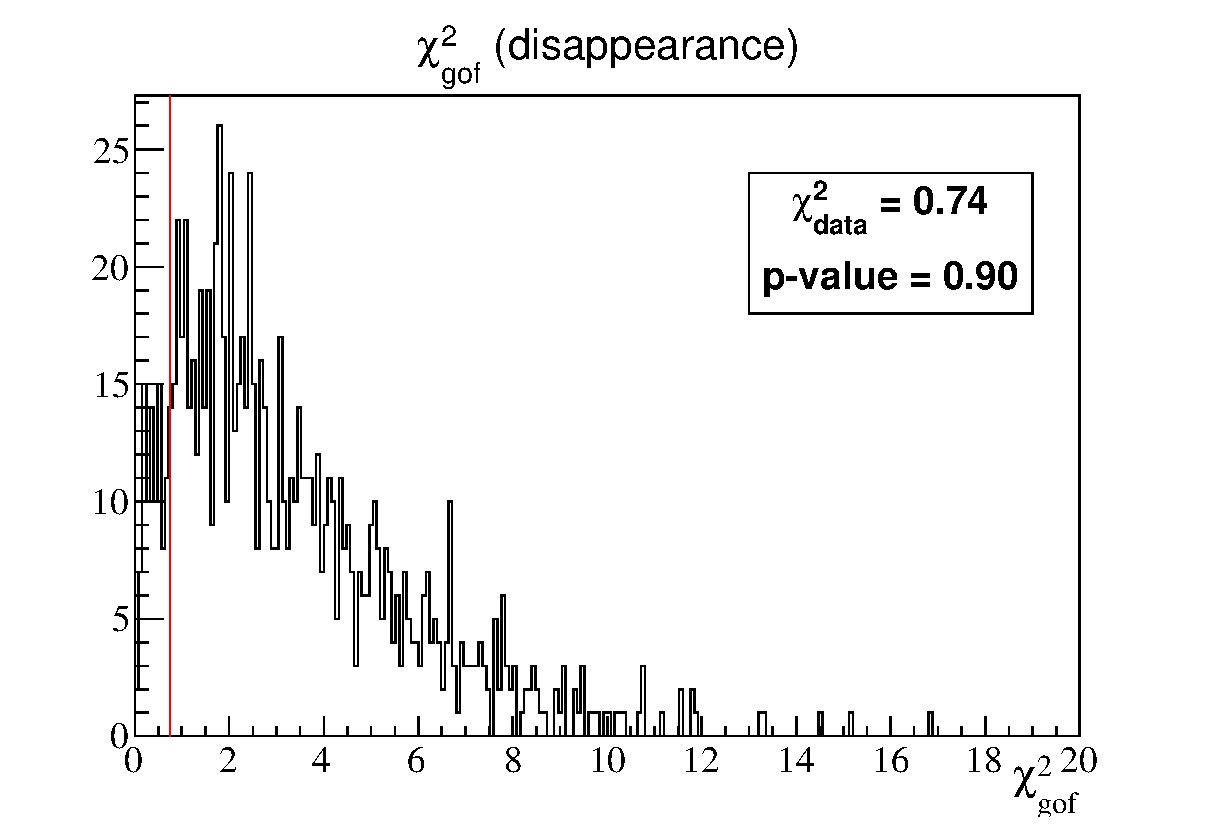
\includegraphics[width=18pc]{./images/results/data_ih_1st_gof_disap_new.eps}
\caption {
  Distribution of $\chi^2_{gof}$
  from 1k toy MC experiments generated at the Run 1+2+3 stand-alone 3-flavour $\nu_{\mu}$ disappearance analysis 
  best-fit oscillation point with Inverted Hierarchy.
  The $\chi^2_{gof}$ value for the Run 1+2+3 data ($\chi^2_{data}$) is highlighted.
  All $\chi^2_{gof}$ values were computed 
  using the 5 (single $\mu$-like ring) 
  reconstructed energy binning scheme described in Sec.\ \ref{sec:goodness_of_fit}.
}
\label{fig:run123_gofchisq_disapp_ih}
\end{minipage}
\hspace{0.03\linewidth}
\begin{minipage}[t]{0.46\linewidth}
\center
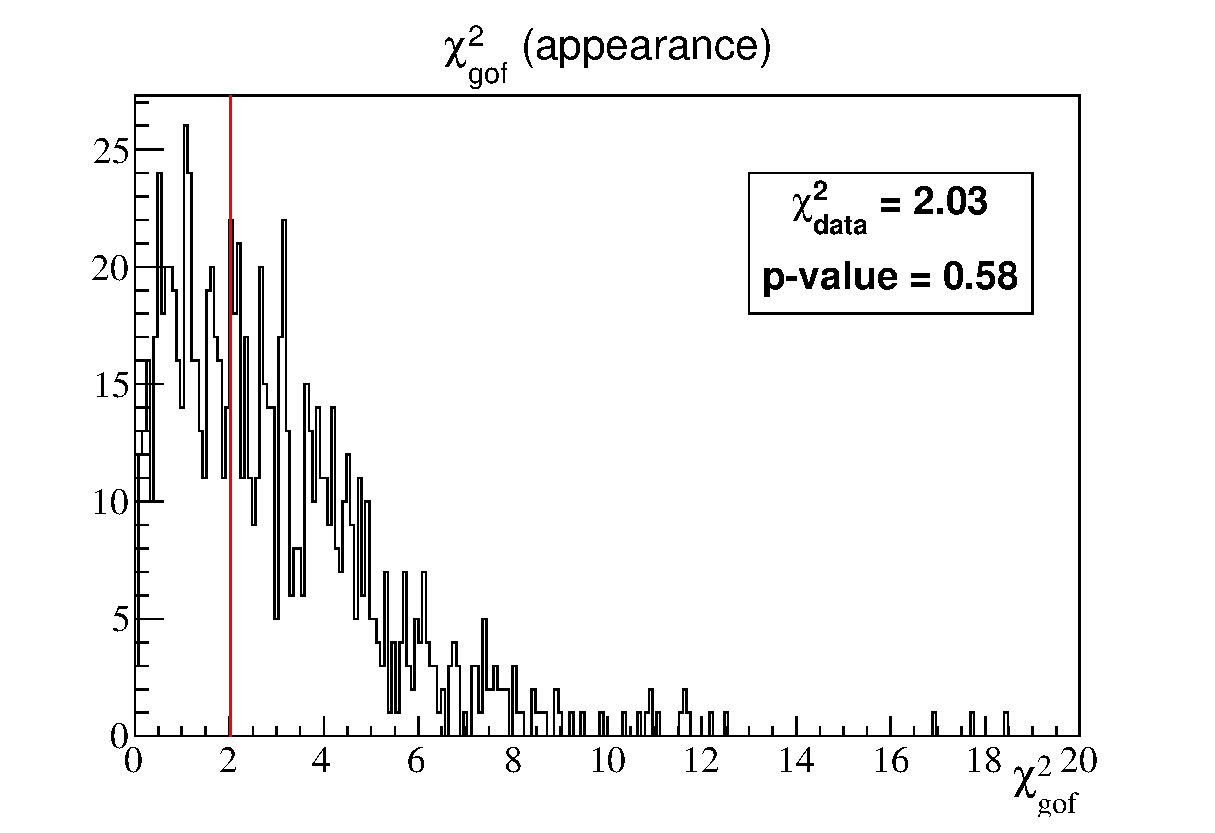
\includegraphics[width=18pc]{./images/results/data_ih_1st_gof_app_new.eps}
\caption {
  Distribution of $\chi^2_{gof}$
  from 1k toy MC experiments generated at the Run 1+2+3 stand-alone 3-flavour $\nu_{e}$ appearance analysis 
  best-fit oscillation point with Inverted Hierarchy.
  The $\chi^2_{gof}$ value for the Run 1+2+3 data ($\chi^2_{data}$) is highlighted.
  All $\chi^2_{gof}$ values were computed 
  using the 3 (single e-like ring) 
  reconstructed energy binning scheme  as described in Sec.\ \ref{sec:goodness_of_fit}.
}
\label{fig:run123_gofchisq_app_ih}
\end{minipage}

\end{figure*}




%...........................................................
%
% Best-fit spectra from the joint-analysis and stand-alone analyses 
% Binning used in the fit
%

\begin{figure*}[htb]

\begin{minipage}[t]{0.98\linewidth}
\center
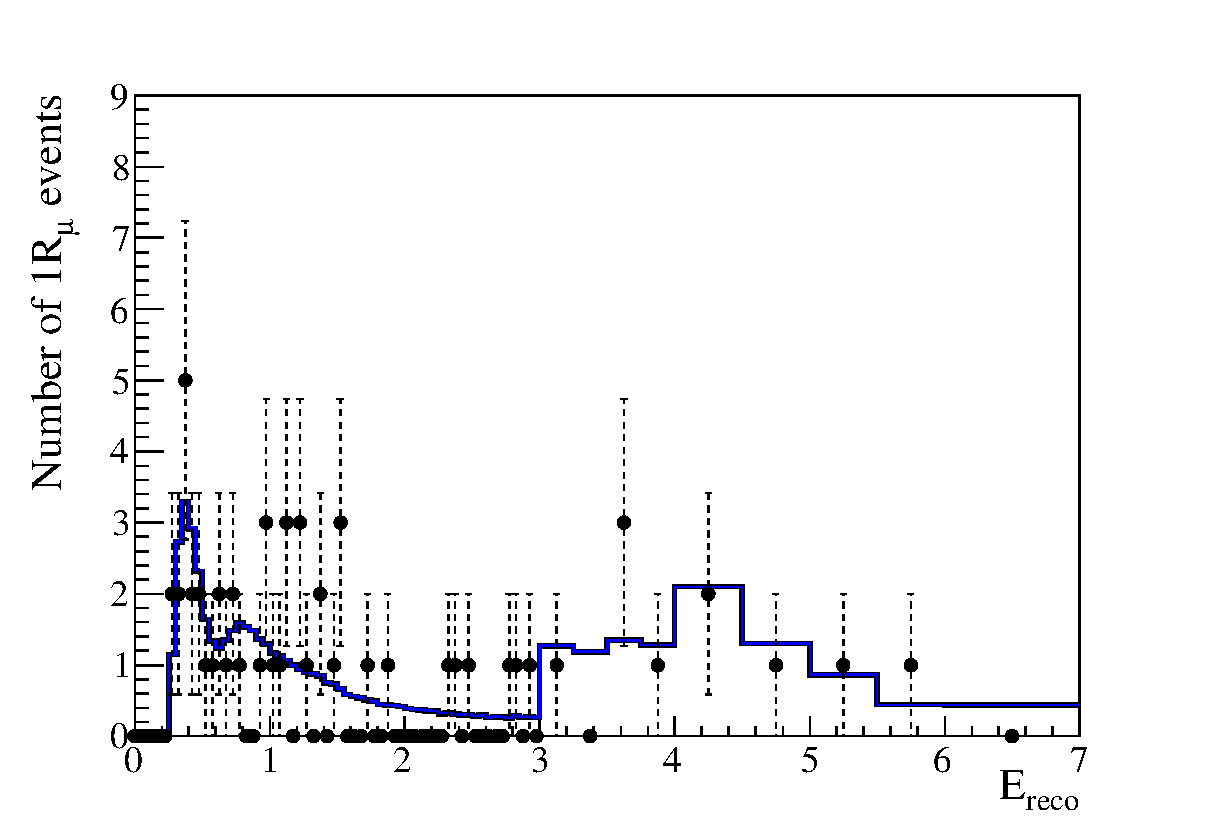
\includegraphics[width=28pc]{./images/results/data_nh_1st_1Rmu.eps}
\caption {
  Run 1+2+3 best-fit single $\mu$-like ring event reconstructed energy spectrum for the fit with Normal Hierarchy
  (black: joint 3-flavour oscillation analysis, blue: stand-alone $\nu_{\mu}$ disappearance analysis).
  The distributions are shown with the binning used in the fit.
}
\label{fig:run123_1Rmu_bestfit_spectrum_nh}
\end{minipage}

\vfill
\vspace*{0.7cm}

\begin{minipage}[t]{0.98\linewidth}
\center
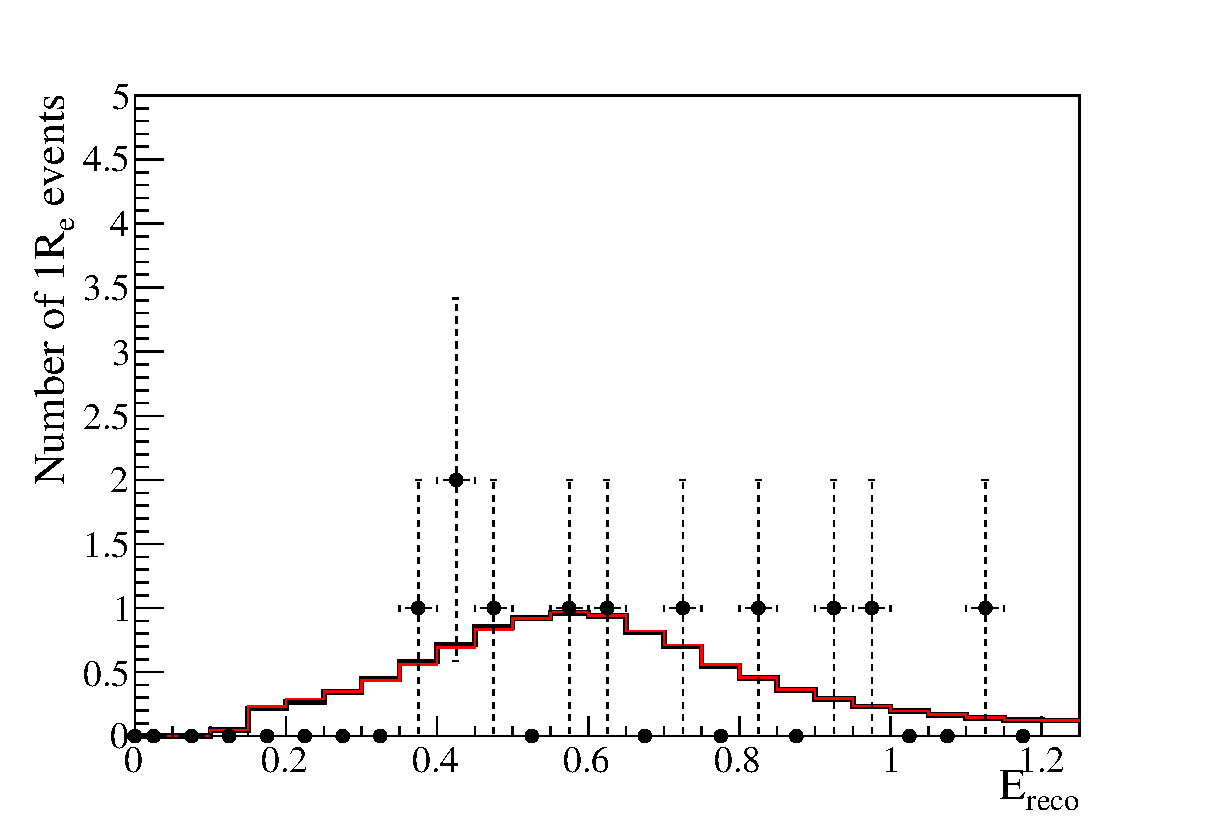
\includegraphics[width=28pc]{./images//results/data_nh_1st_1Re.eps}
\caption {
  Run 1+2+3 best-fit single e-like ring event reconstructed energy spectrum for the fit with Normal Hierarchy
  (black: joint 3-flavour oscillation analysis, red: stand-alone $\nu_{e}$ disappearance analysis).
  The distributions are shown with the binning used in the fit.
}
\label{fig:run123_1Re_bestfit_spectrum_nh}
\end{minipage}

\end{figure*}

\begin{figure*}[htb]

\begin{minipage}[t]{0.98\linewidth}
\center
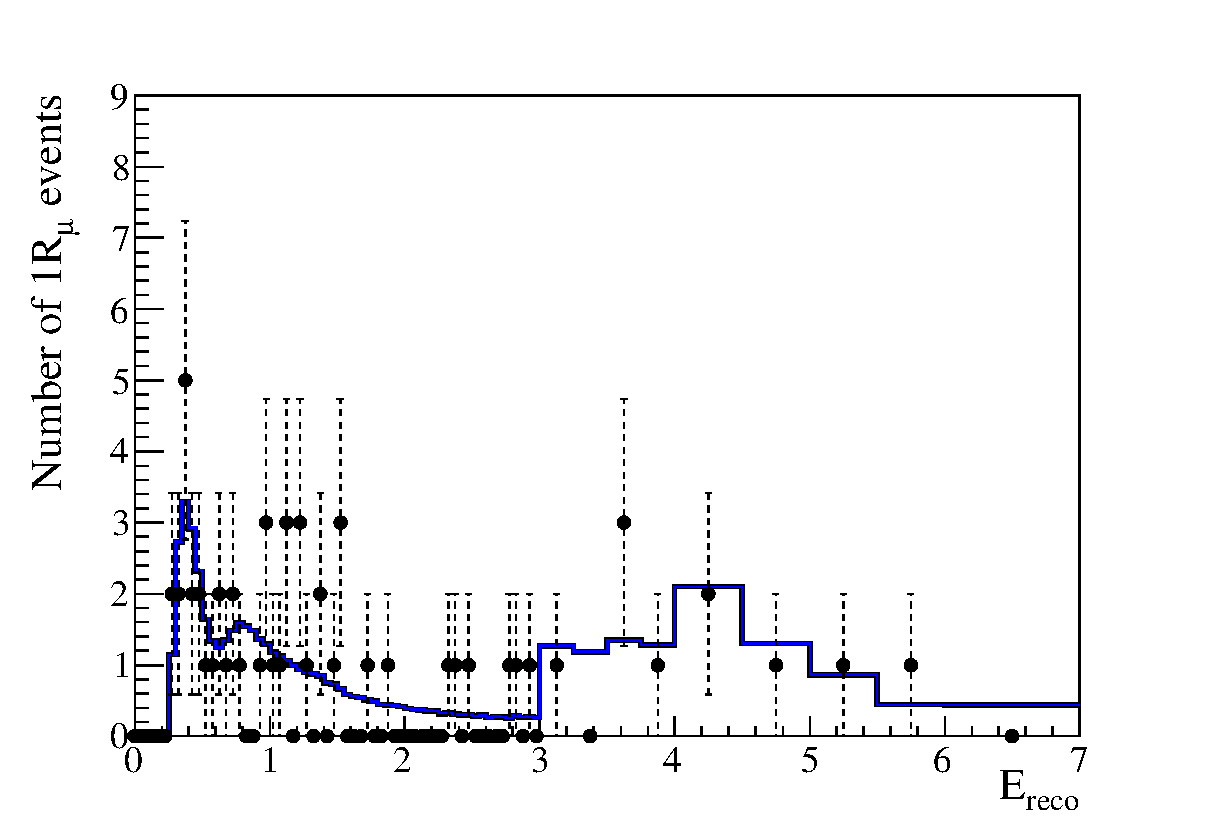
\includegraphics[width=28pc]{./images//results/data_ih_1st_1Rmu.eps}
\caption {
  Run 1+2+3 best-fit single $\mu$-like ring event reconstructed energy spectrum for the fit with Inverted Hierarchy
  (black: joint 3-flavour oscillation analysis, blue: stand-alone $\nu_{\mu}$ disappearance analysis).
  The distributions are shown with the binning used in the fit.
}
\label{fig:run123_1Rmu_bestfit_spectrum_ih}
\end{minipage}

\vfill
\vspace*{0.7cm}

\begin{minipage}[t]{0.98\linewidth}
\center
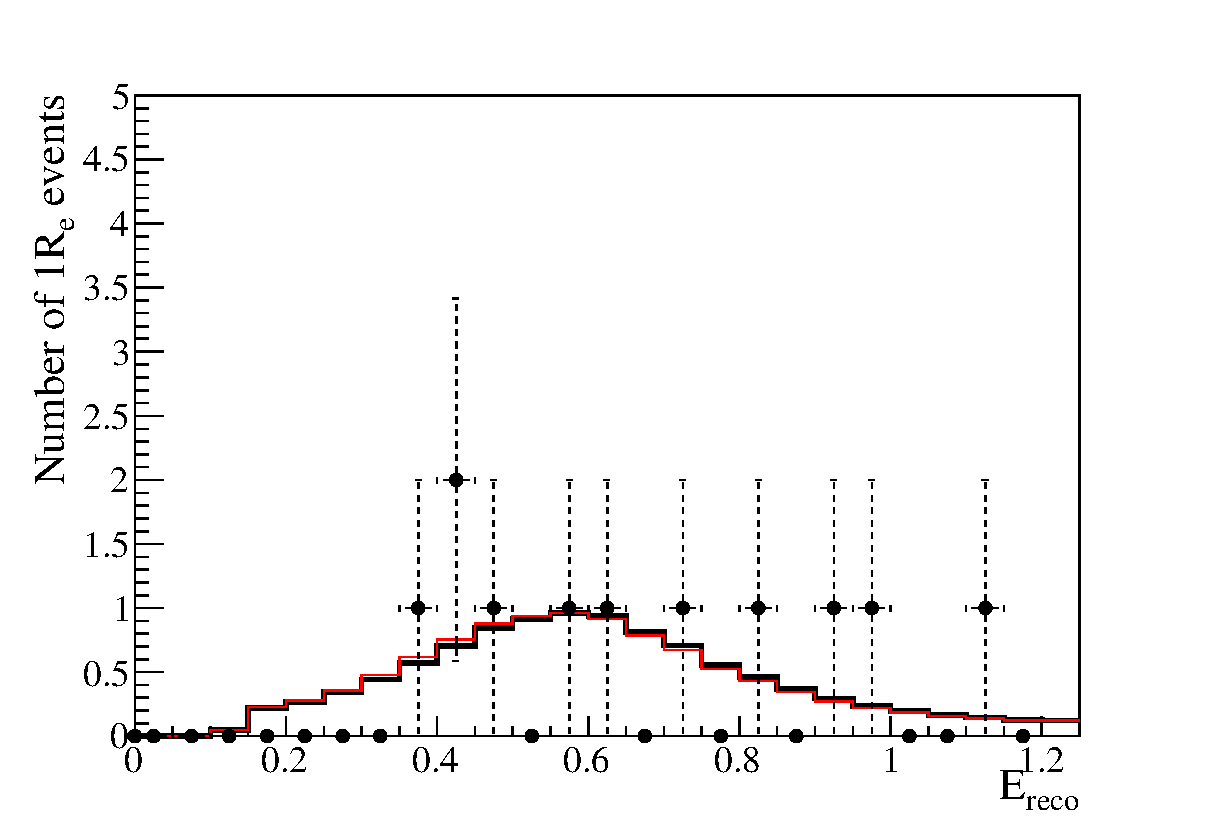
\includegraphics[width=28pc]{./images//results/data_ih_1st_1Re.eps}
\caption {
  Run 1+2+3 best-fit single e-like ring event reconstructed energy spectrum for the fit with inverted Hierarchy
  (black: joint 3-flavour oscillation analysis, red: stand-alone $\nu_{e}$ disappearance analysis).
  The distributions are shown with the binning used in the fit.
}
\label{fig:run123_1Re_bestfit_spectrum_ih}
\end{minipage}

\end{figure*}


%...........................................................
%
% Best-fit spectra from the joint-analysis and stand-alone analyses 
% Coarse binning.
%

\begin{figure*}[htb]

\begin{minipage}[t]{0.98\linewidth}
\center
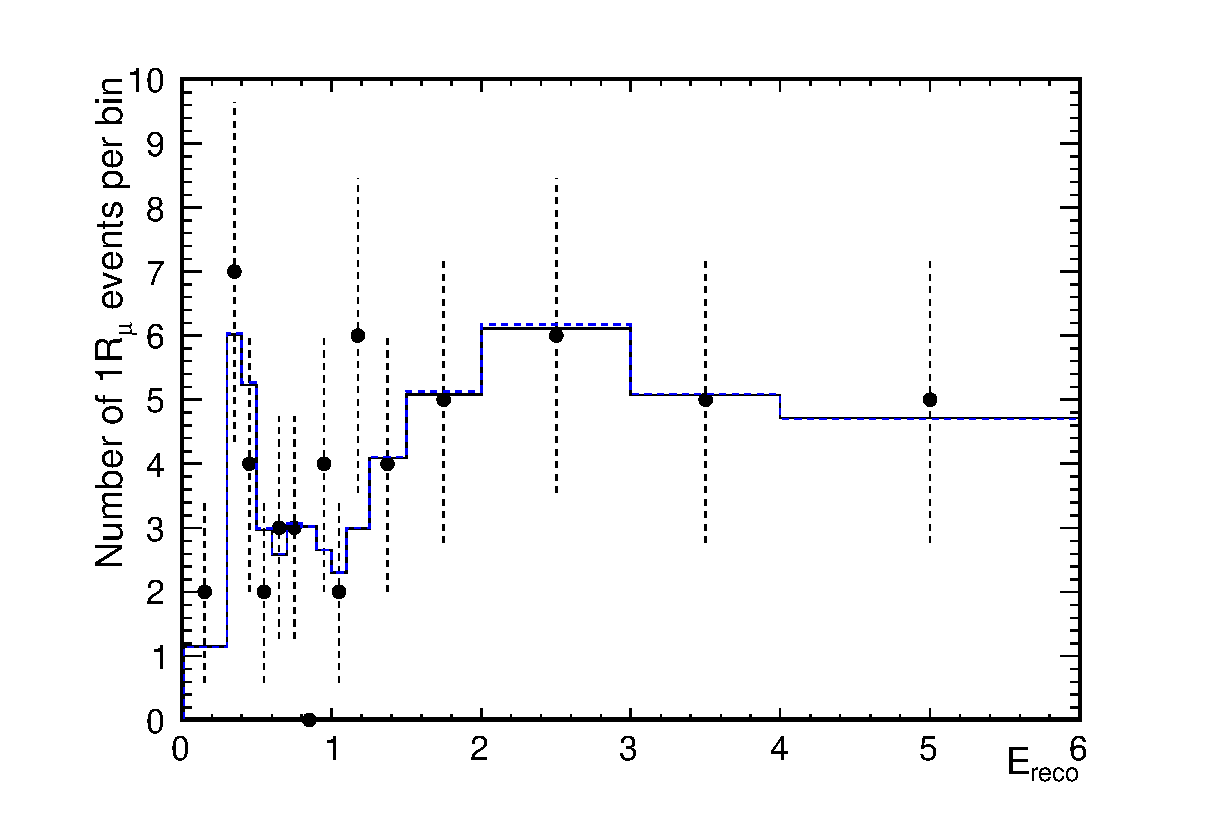
\includegraphics[width=28pc]{./images/results/bestfit_spectra_1Rmu_nh_coarse.eps}
\caption {
  Run 1+2+3 best-fit single $\mu$-like ring event reconstructed energy spectrum for the fit with Normal Hierarchy
  (black: joint 3-flavour oscillation analysis, blue: stand-alone $\nu_{\mu}$ disappearance analysis).
  The distributions are shown with the coarse binning defined in the main text.
}
\label{fig:run123_1Rmu_bestfit_spectrum_nh_coarse}
\end{minipage}

\vfill
\vspace*{0.7cm}

\begin{minipage}[t]{0.98\linewidth}
\center
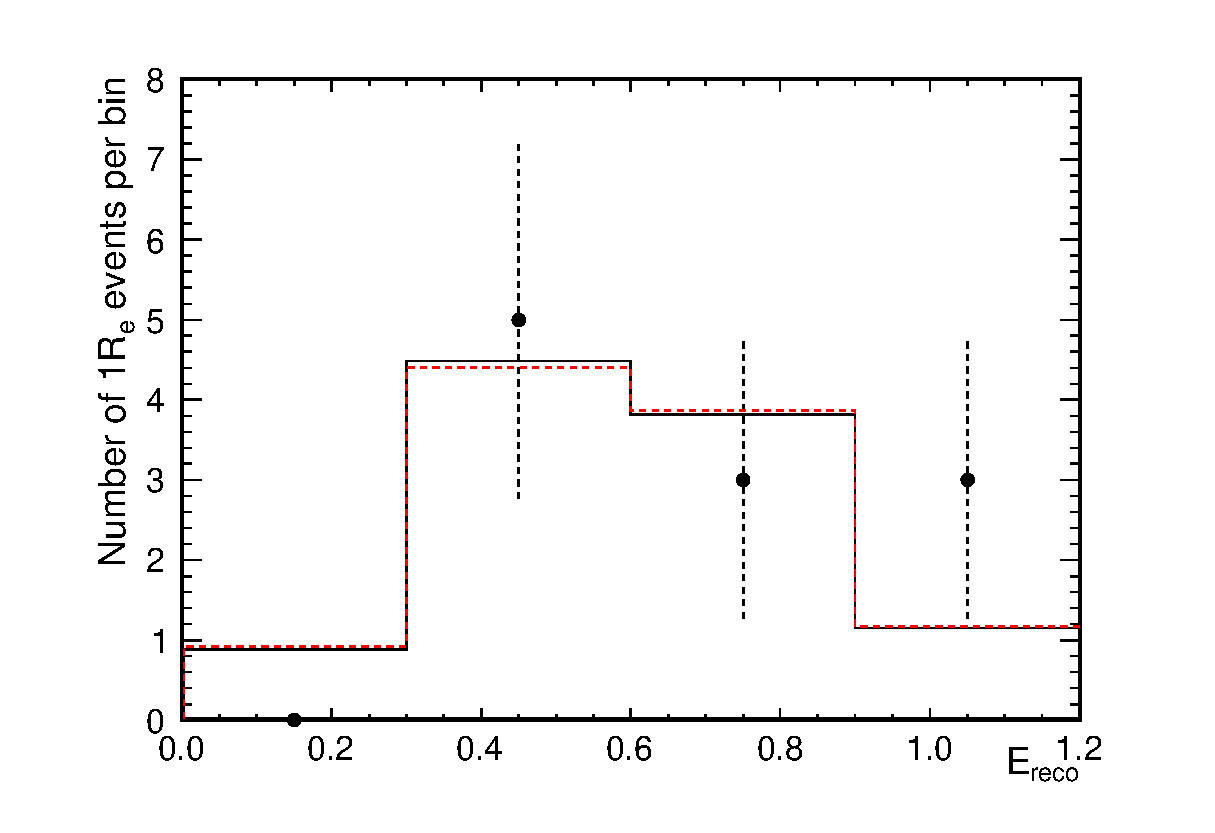
\includegraphics[width=28pc]{./images//results/bestfit_spectra_1Re_nh_coarse.eps}
\caption {
  Run 1+2+3 best-fit single e-like ring event reconstructed energy spectrum for the fit with Normal Hierarchy
  (black: joint 3-flavour oscillation analysis, red: stand-alone $\nu_{e}$ disappearance analysis).
  The distributions are shown with the coarse binning defined in the main text.
}
\label{fig:run123_1Re_bestfit_spectrum_nh_coarse}
\end{minipage}

\end{figure*}

\begin{figure*}[htb]

\begin{minipage}[t]{0.98\linewidth}
\center
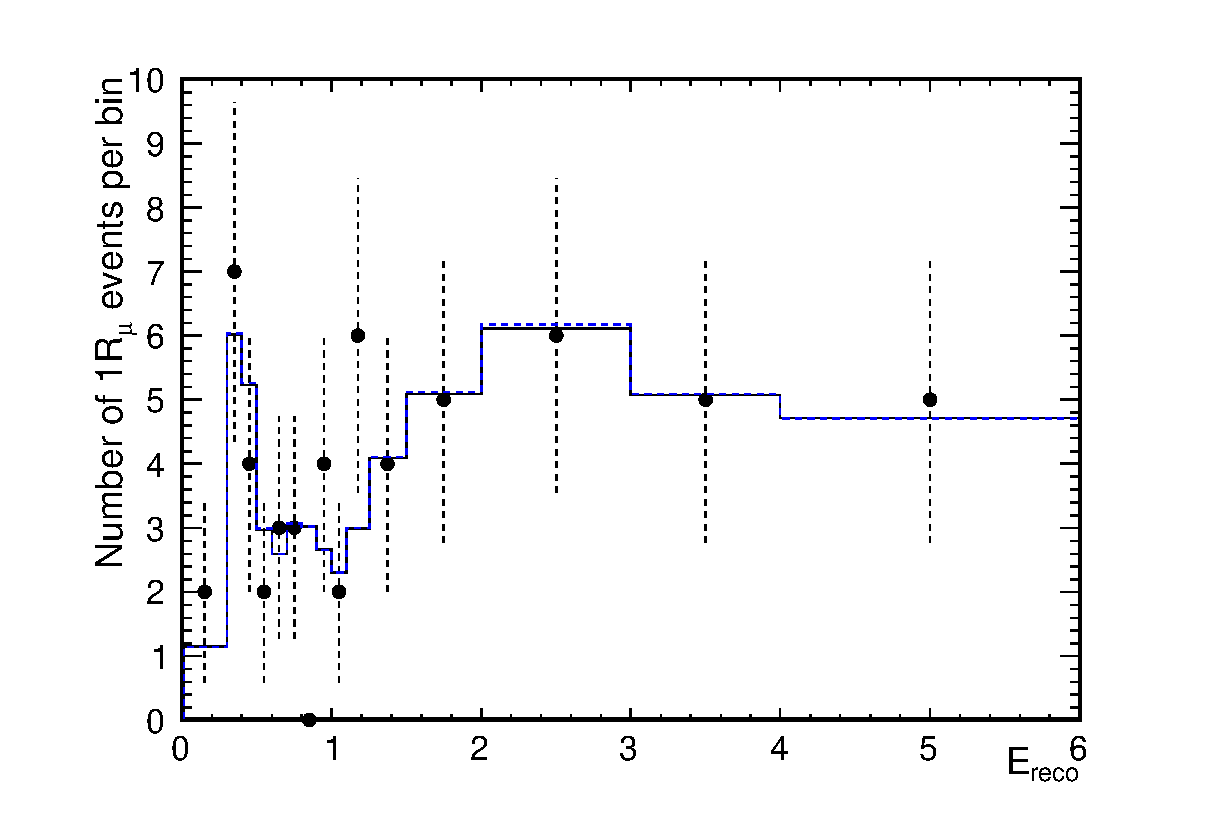
\includegraphics[width=28pc]{./images//results/bestfit_spectra_1Rmu_ih_coarse.eps}
\caption {
  Run 1+2+3 best-fit single $\mu$-like ring event reconstructed energy spectrum for the fit with Inverted Hierarchy
  (black: joint 3-flavour oscillation analysis, blue: stand-alone $\nu_{\mu}$ disappearance analysis).
  The distributions are shown with the coarse binning defined in the main text.
}
\label{fig:run123_1Rmu_bestfit_spectrum_ih_coarse}
\end{minipage}

\vfill
\vspace*{0.7cm}

\begin{minipage}[t]{0.98\linewidth}
\center
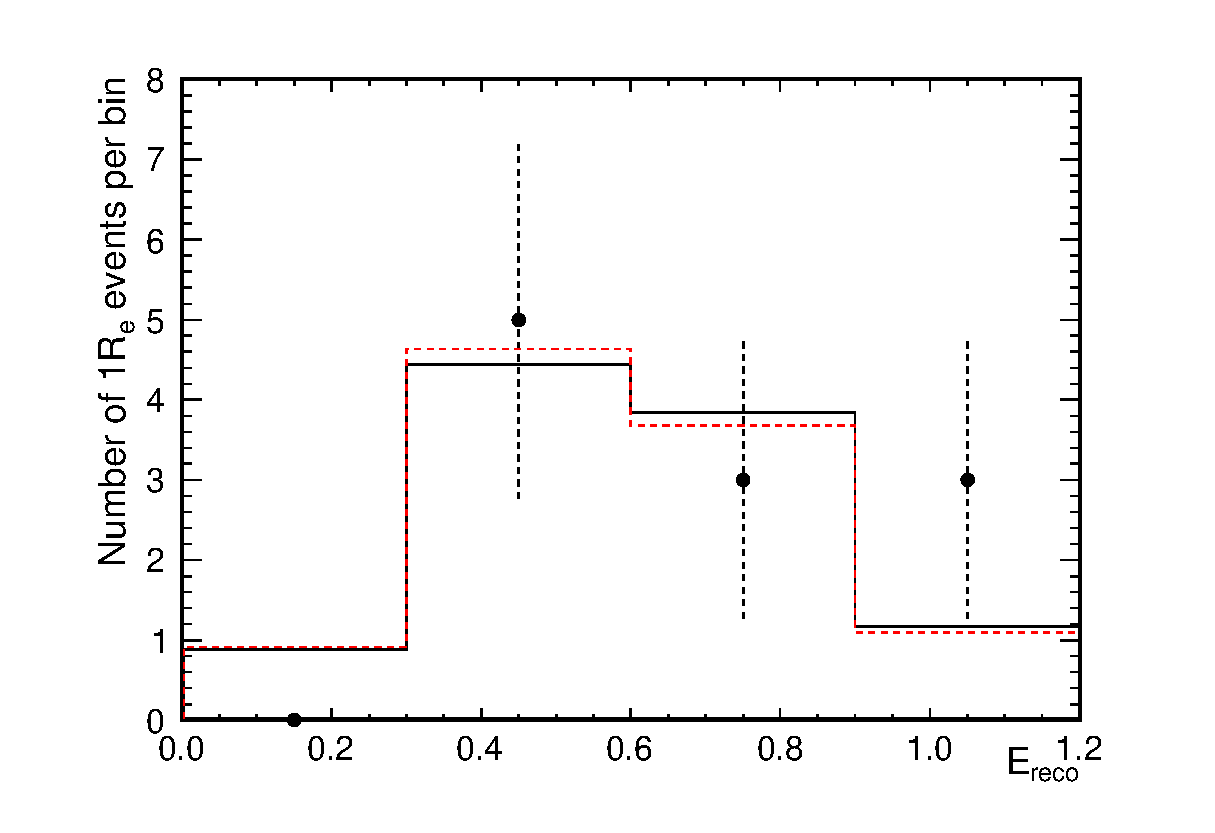
\includegraphics[width=28pc]{./images//results/bestfit_spectra_1Re_ih_coarse.eps}
\caption {
  Run 1+2+3 best-fit single e-like ring event reconstructed energy spectrum for the fit with inverted Hierarchy
  (black: joint 3-flavour oscillation analysis, red: stand-alone $\nu_{e}$ disappearance analysis).
  The distributions are shown with the coarse binning defined in the main text.
}
\label{fig:run123_1Re_bestfit_spectrum_ih_coarse}
\end{minipage}

\end{figure*}


%...........................................................
%
% Ratio of the best-fit spectra from the joint-analysis over the
% best-fit spectra from the stand-alone analyses.
% Binning used in the fit
%

\begin{figure*}[htb]

\begin{minipage}[t]{0.98\linewidth}
\center
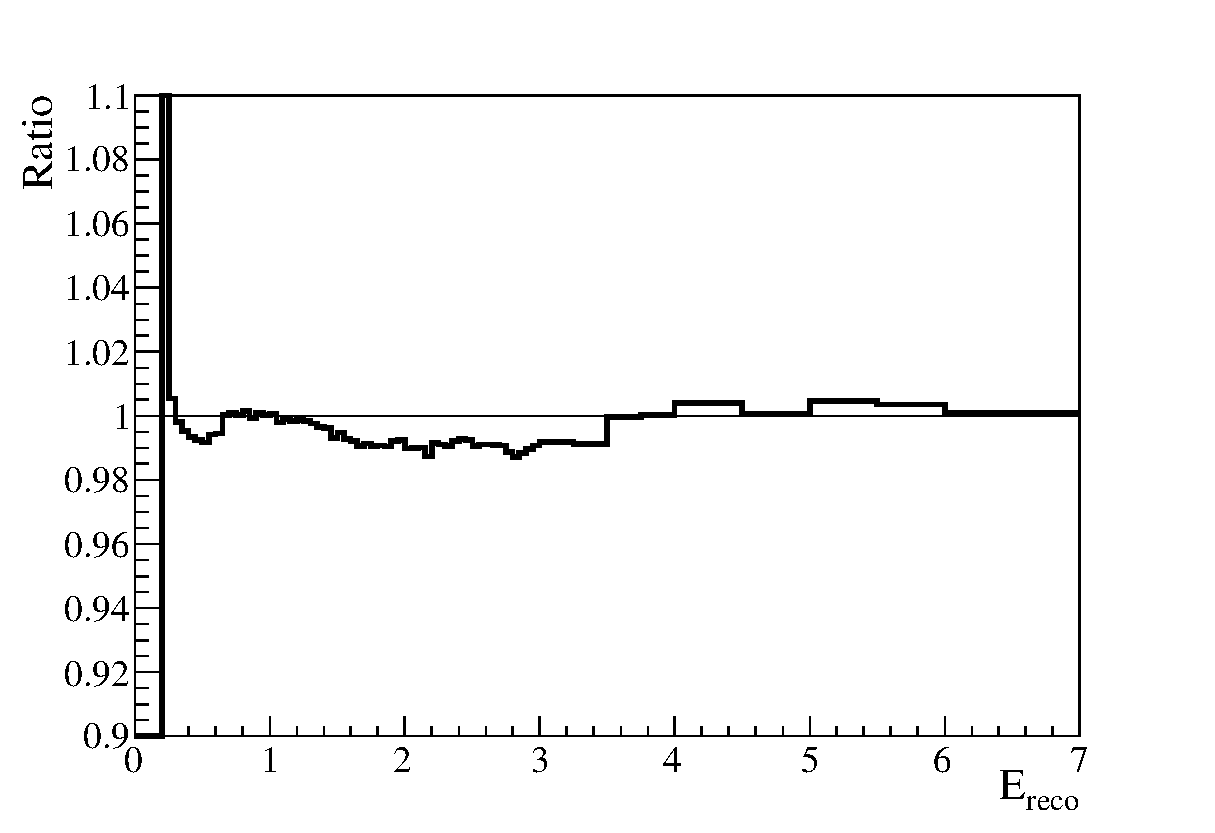
\includegraphics[width=28pc]{./images/results/Ratio_data_nh_1st_1Rmu.eps}
\caption {
  Ratio of the Run 1+2+3 best-fit single $\mu$-like ring event reconstructed energy spectra
  obtained from the joint 3-flavour oscillation and the stand-alone $\nu_{\mu}$ disappearance analyses
  (joint / stand-alone) with Normal Hierarchy.
  The distributions are shown with the binning used in the fit.
}
\label{fig:run123_1Rmu_bestfit_spectrum_ratio_nh}
\end{minipage}

\vfill
\vspace*{0.7cm}

\begin{minipage}[t]{0.98\linewidth}
\center
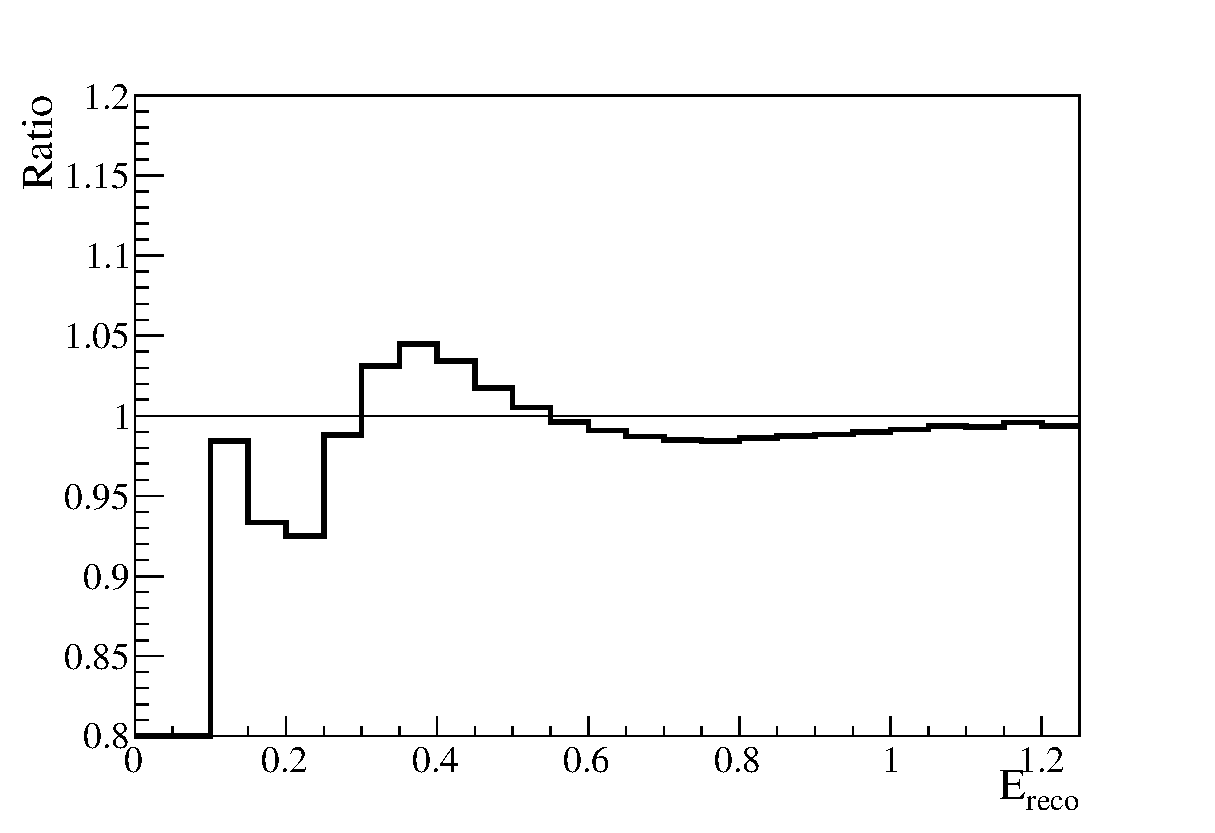
\includegraphics[width=28pc]{./images/results/Ratio_data_nh_1st_1Re.eps}
\caption {
  Ratio of the Run 1+2+3 best-fit single e-like ring event reconstructed energy spectra
  obtained from the joint 3-flavour oscillation and the stand-alone $\nu_{e}$ appearance analyses.
  (joint / stand-alone) with Normal Hierarchy.
  The distributions are shown with the binning used in the fit.
}
\label{fig:run123_1Re_bestfit_spectrum_ratio_nh}
\end{minipage}

\end{figure*}

\begin{figure*}[htb]

\begin{minipage}[t]{0.98\linewidth}
\center
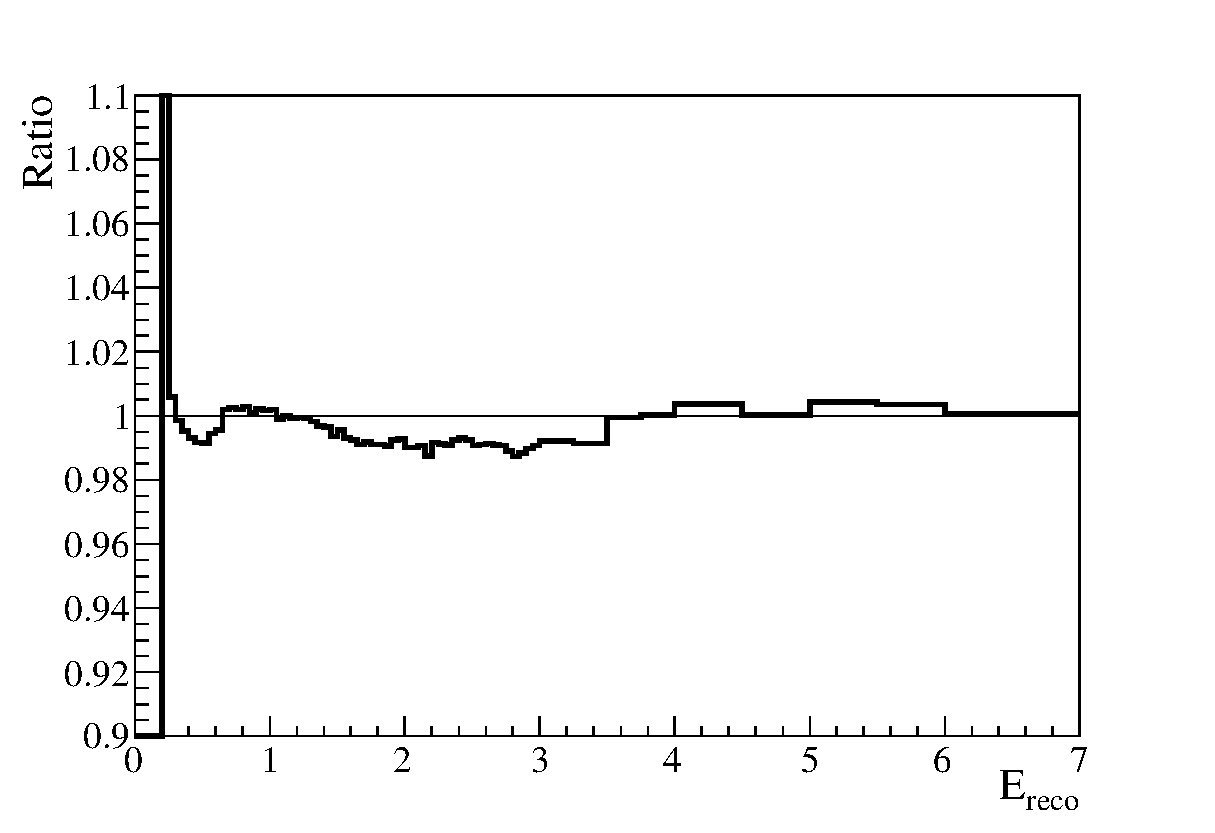
\includegraphics[width=28pc]{./images/results/Ratio_data_ih_1st_1Rmu.eps}
\caption {
  Ratio of the Run 1+2+3 best-fit single $\mu$-like ring event reconstructed energy spectra
  obtained from the joint 3-flavour oscillation and the stand-alone $\nu_{\mu}$ disappearance analyses
  (joint / stand-alone) with Inverted Hierarchy.
  The distributions are shown with the binning used in the fit.
}
\label{fig:run123_1Rmu_bestfit_spectrum_ratio_ih}
\end{minipage}

\vfill
\vspace*{0.7cm}

\begin{minipage}[t]{0.98\linewidth}
\center
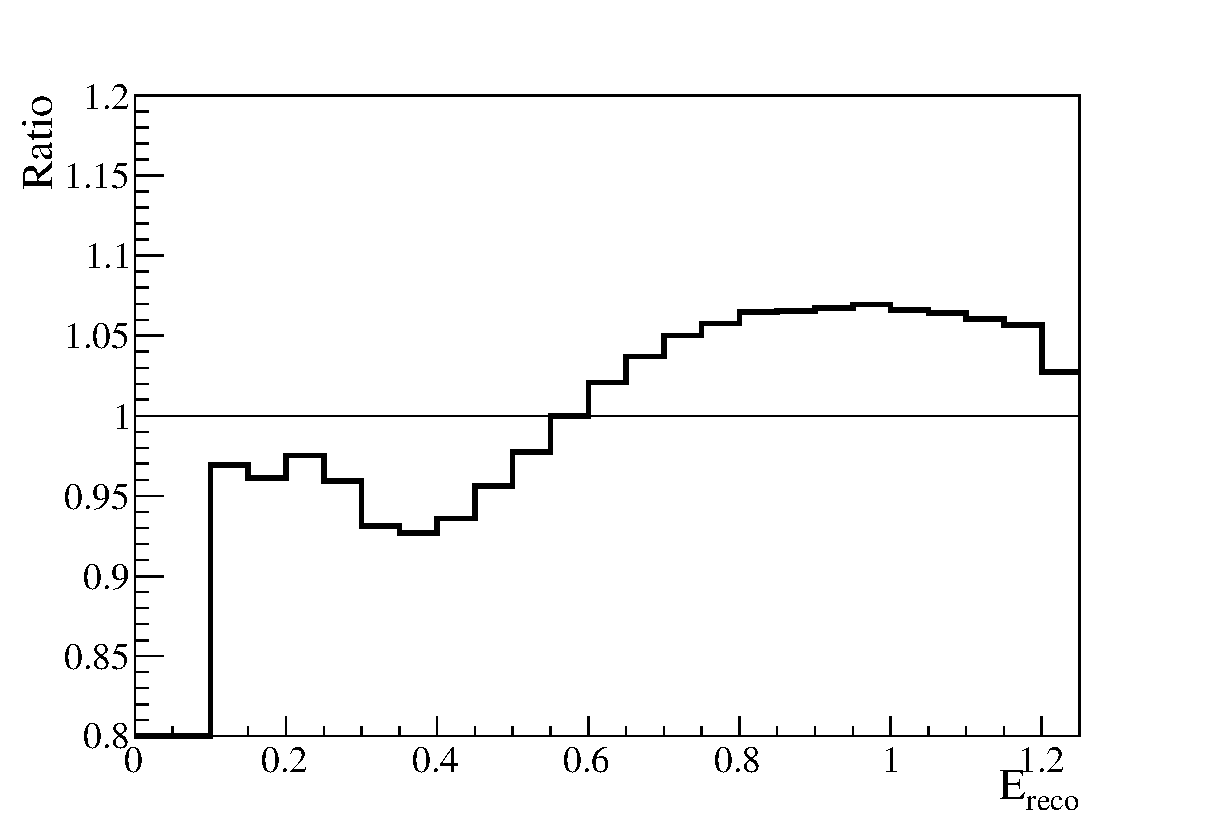
\includegraphics[width=28pc]{./images/results/Ratio_data_ih_1st_1Re.eps}
\caption {
  Ratio of the Run 1+2+3 best-fit single e-like ring event reconstructed energy spectra
  obtained from the joint 3-flavour oscillation and the stand-alone $\nu_{e}$ appearance analyses.
  (joint / stand-alone) with Inverted Hierarchy.
  The distributions are shown with the binning used in the fit.
}
\label{fig:run123_1Re_bestfit_spectrum_ratio_ih}
\end{minipage}

\end{figure*}


%...........................................................
%
% marginalized (1D) delta\chisq distributions
%

\begin{figure*}[htb]

\begin{minipage}[t]{0.45\linewidth}
\center
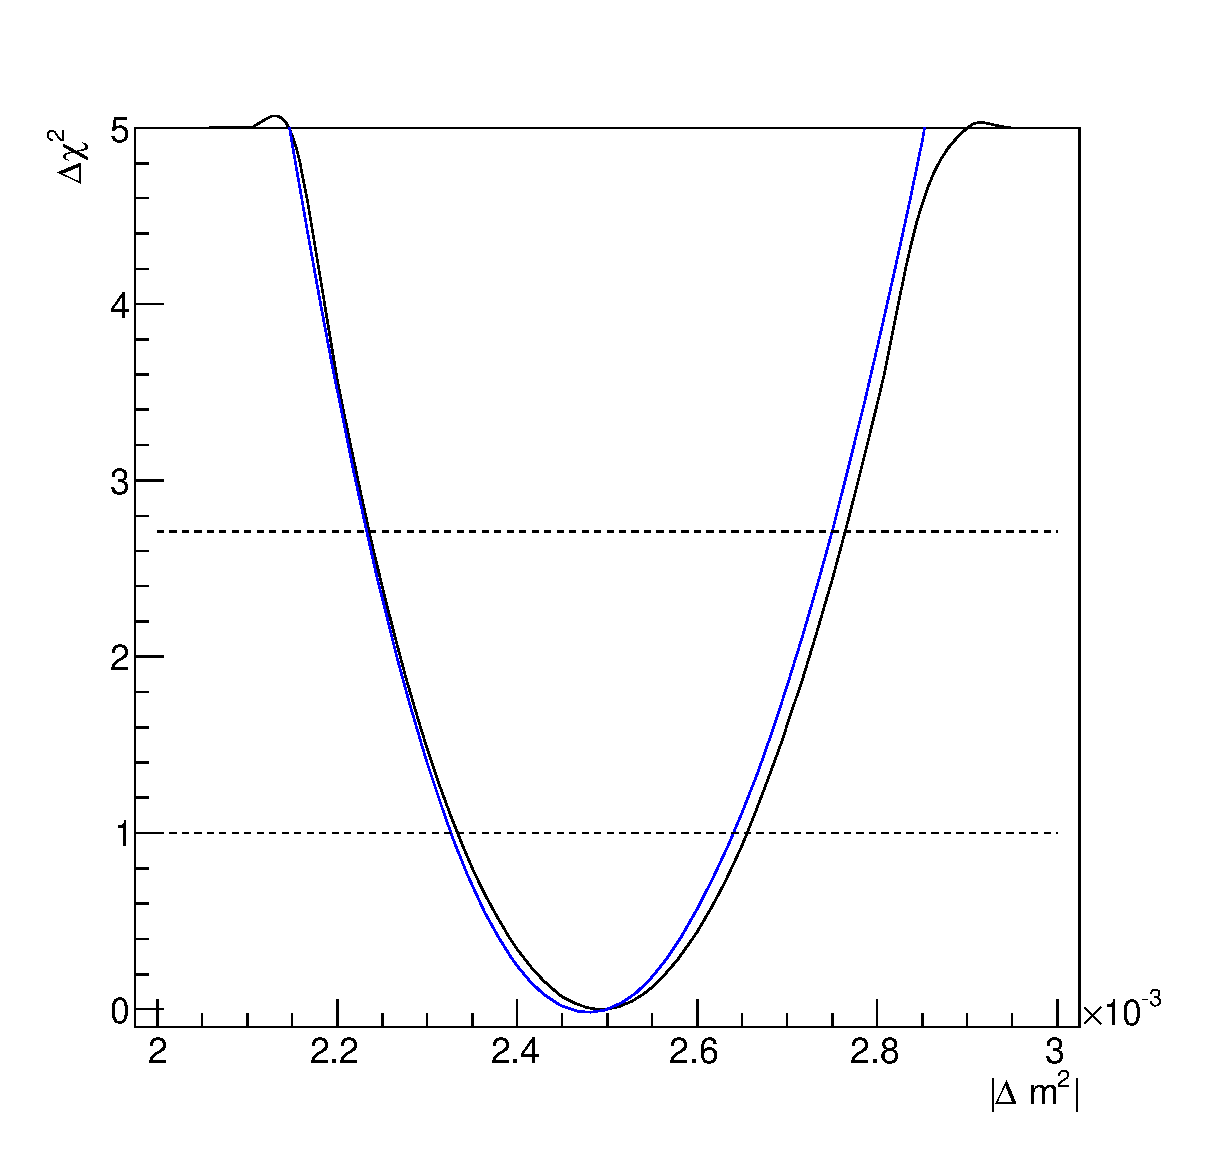
\includegraphics[width=18pc]{./images/results/data_chisq_dm23sq_global_min_new.eps}
\caption {
  $\Delta\chi^2$ as function of $|\Delta m^{2}|$ from the analysis of the Run 1+2+3 dataset
  comparing the joint analysis (black) with the stand-alone $\nu_{\mu}$ disappearance (blue)
  for Normal Hierarchy. 
  At each point, $\chi^2$ was minimized with respect to
  all oscillation parameters not shown (and not considered to be fixed)
  and all relevant nuisance parameters.
}
\label{fig:run123_dchisq_Dmsq_nh}
\end{minipage}
\hspace{0.04\linewidth}
\begin{minipage}[t]{0.45\linewidth}
\center
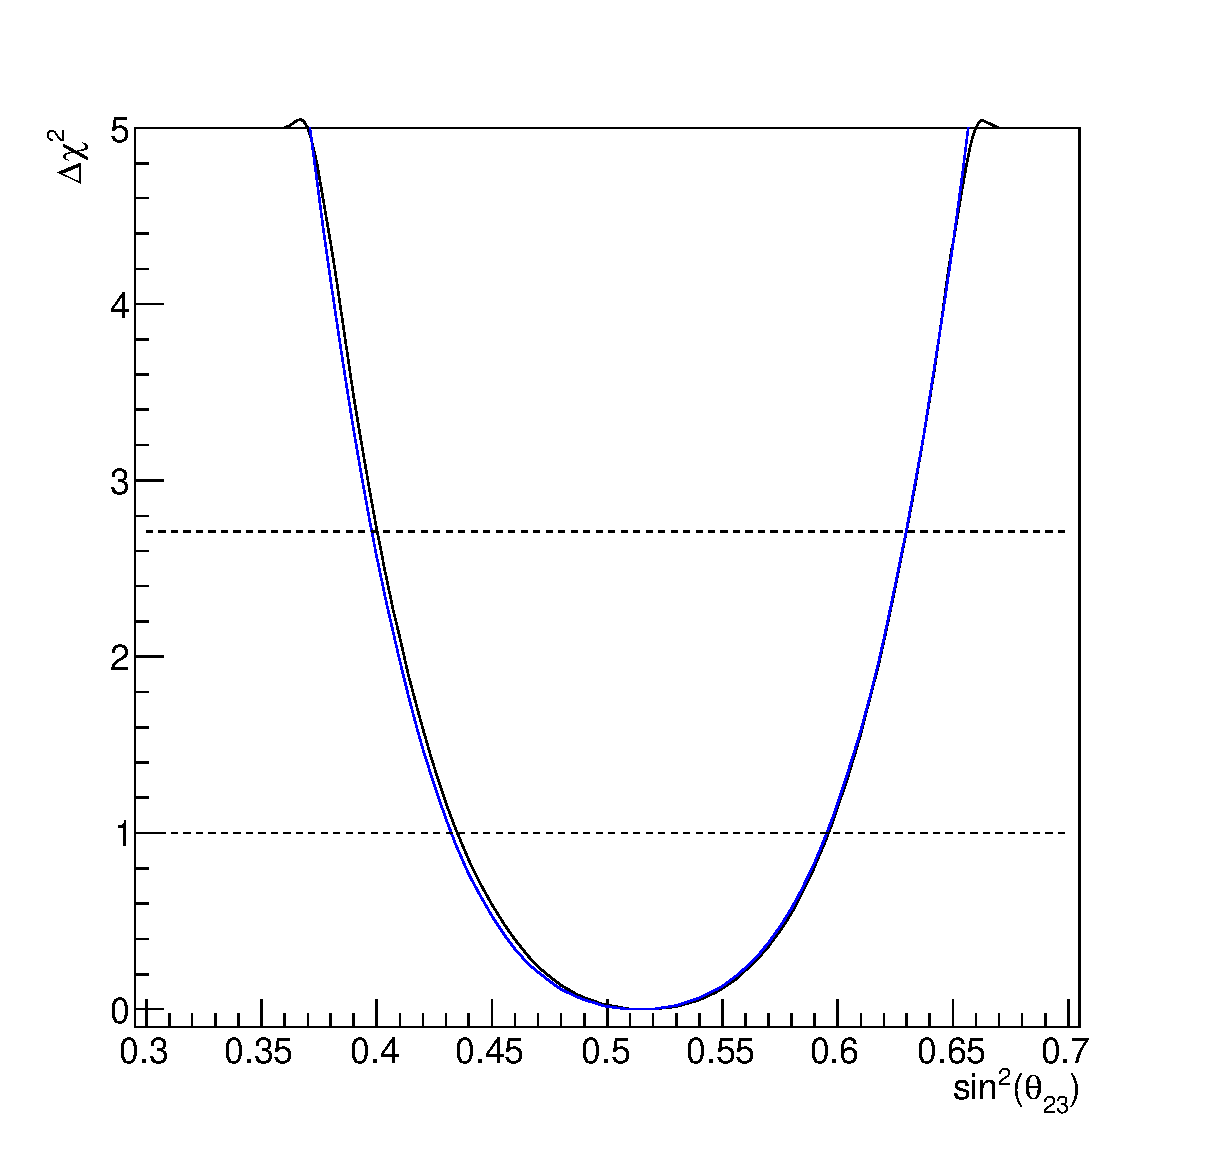
\includegraphics[width=18pc]{./images/results/data_chisq_theta23_global_min_new.eps}
\caption {
  $\Delta\chi^2$ as function of $sin^{2}\theta_{23}$ from the analysis of the Run 1+2+3 dataset
   comparing the joint analysis (black) with the stand-alone $\nu_{\mu}$ disappearance (blue)
     for Normal Hierarchy. 	
  At each point, $\chi^2$ was minimized with respect to
  all oscillation parameters not shown (and not considered to be fixed)
  and all relevant nuisance parameters.
}
\label{fig:run123_dchisq_sinsqtheta23_nh}
\end{minipage}

\vfill
\vspace*{0.7cm}

\begin{minipage}[t]{0.45\linewidth}
\center
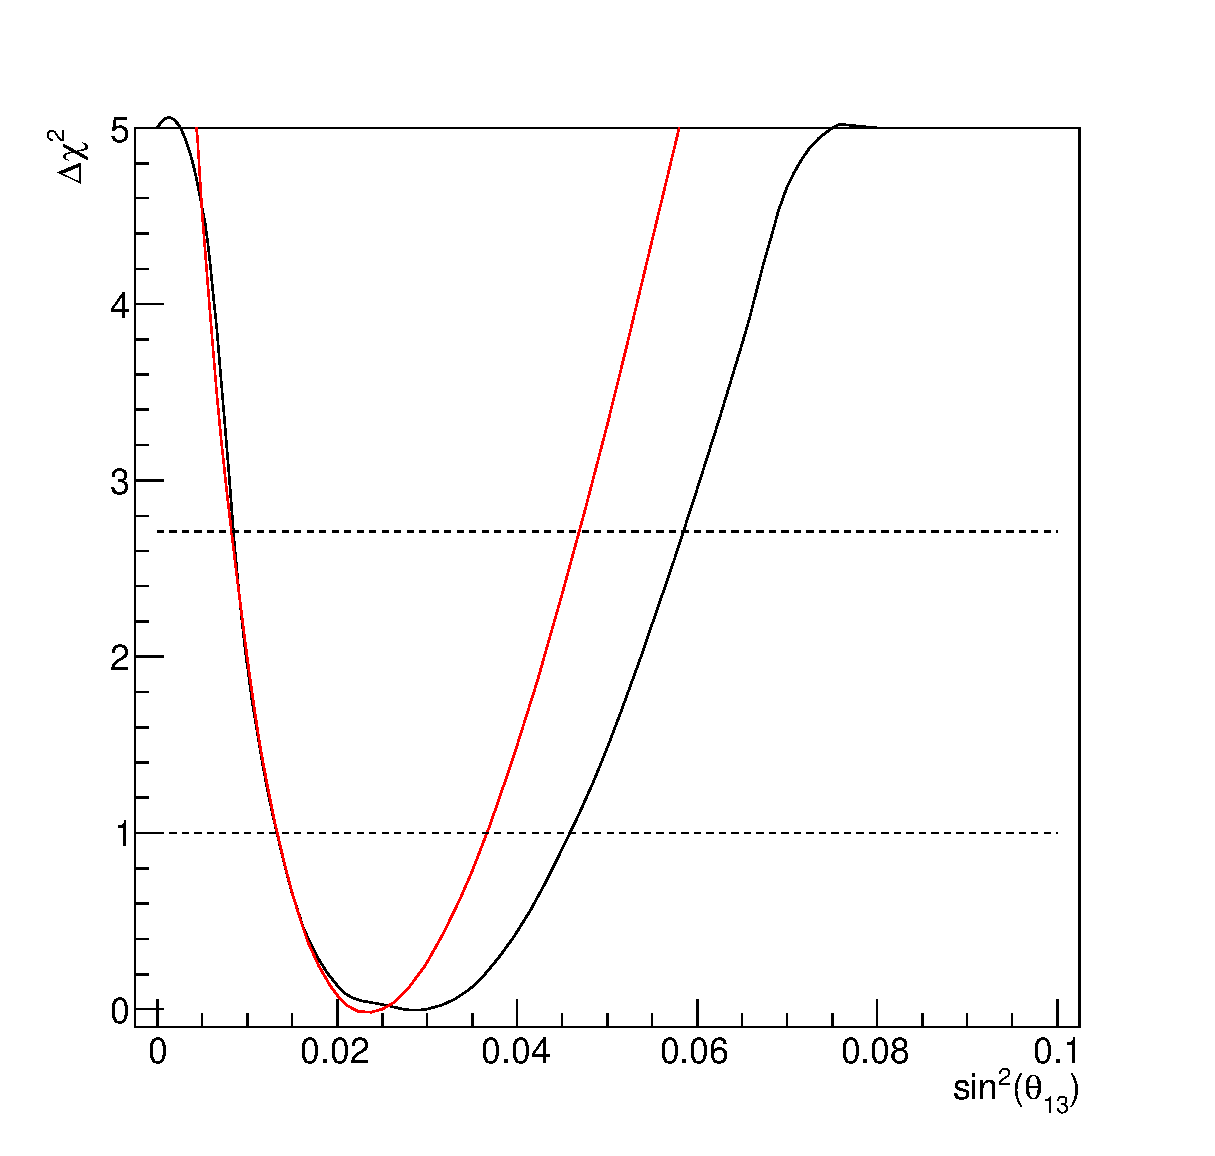
\includegraphics[width=18pc]{./images/results/data_chisq_theta13_global_min_new.eps}
\caption {
  $\Delta\chi^2$ as function of $sin^{2}\theta_{13}$ from the analysis of the Run 1+2+3 dataset
   comparing the joint analysis (black) with the stand-alone $\nu_{e}$ appearance (red)
     for Normal Hierarchy. 
  At each point, $\chi^2$ was minimized with respect to
  all oscillation parameters not shown (and not considered to be fixed)
  and all relevant nuisance parameters.
}
\label{fig:run123_dchisq_sinsqtheta13_nh}
\end{minipage}
\hspace{0.04\linewidth}
\begin{minipage}[t]{0.45\linewidth}
\center
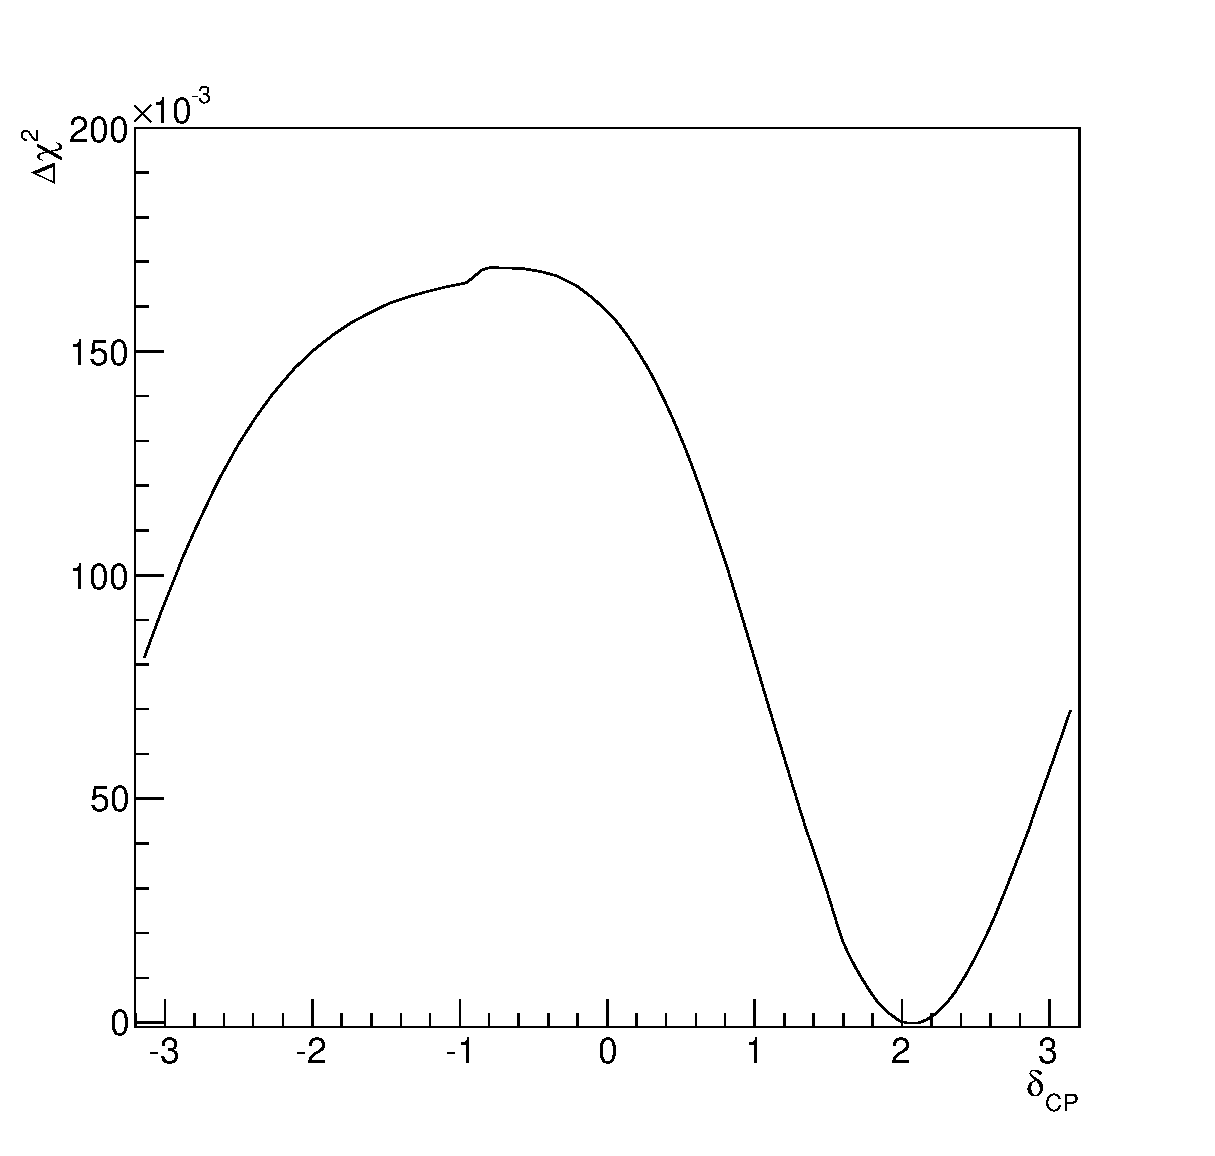
\includegraphics[width=18pc]{./images/results/data_chisq_deltacp_global_min_new.eps}
\caption {
  $\Delta\chi^2$ as function of $\delta_{CP}$ from the analysis of the Run 1+2+3 dataset  for Normal Hierarchy. 
  At each point, $\chi^2$ was minimized with respect to
  all oscillation parameters not shown (and not considered to be fixed)
  and all relevant nuisance parameters.
}
\label{fig:run123_dchisq_deltacp_nh}
\end{minipage}

\end{figure*}

%...........................................................
%
% contours 
% that can be compared with stand-alone analyses
% dmsq - sinsqtheta23, deltacp - sinsqtheta13
%

\begin{figure*}[htb]

\begin{minipage}[t]{0.98\linewidth}
\center
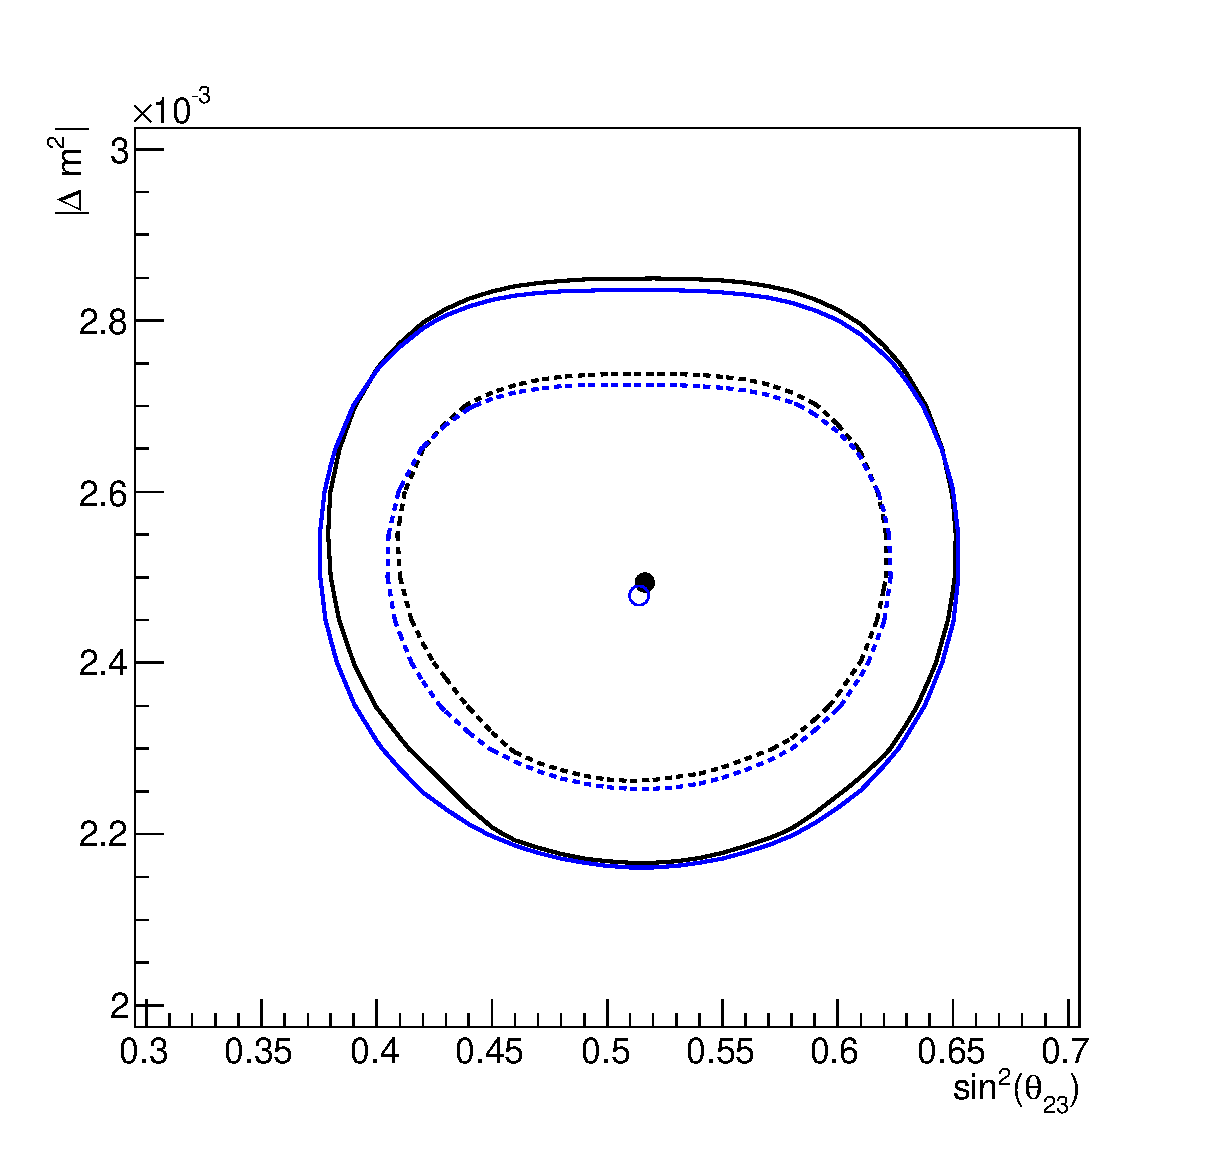
\includegraphics[width=22pc]{./images/results/data_chisq_theta23_dm23sq_global_min_new.eps}
\caption {
  68\% (dashed lines) and 90\% (solid lines) CL regions in ($sin^{2}\theta_{23}$, $|\Delta m^{2}|$) space 
  from the analysis of the Run 1+2+3 dataset
   comparing the joint analysis (black) with the stand-alone $\nu_{\mu}$ disappearance (blue)
     for Normal Hierarchy. 	
  At each point, $\chi^2$ was minimized with respect to
  all oscillation parameters not shown (and not considered to be fixed)
  and all relevant nuisance parameters.
}
\label{fig:run123_confreg_sinsqtheta23_Dmsq_nh}
\end{minipage}
\begin{minipage}[t]{0.98\linewidth}
\center
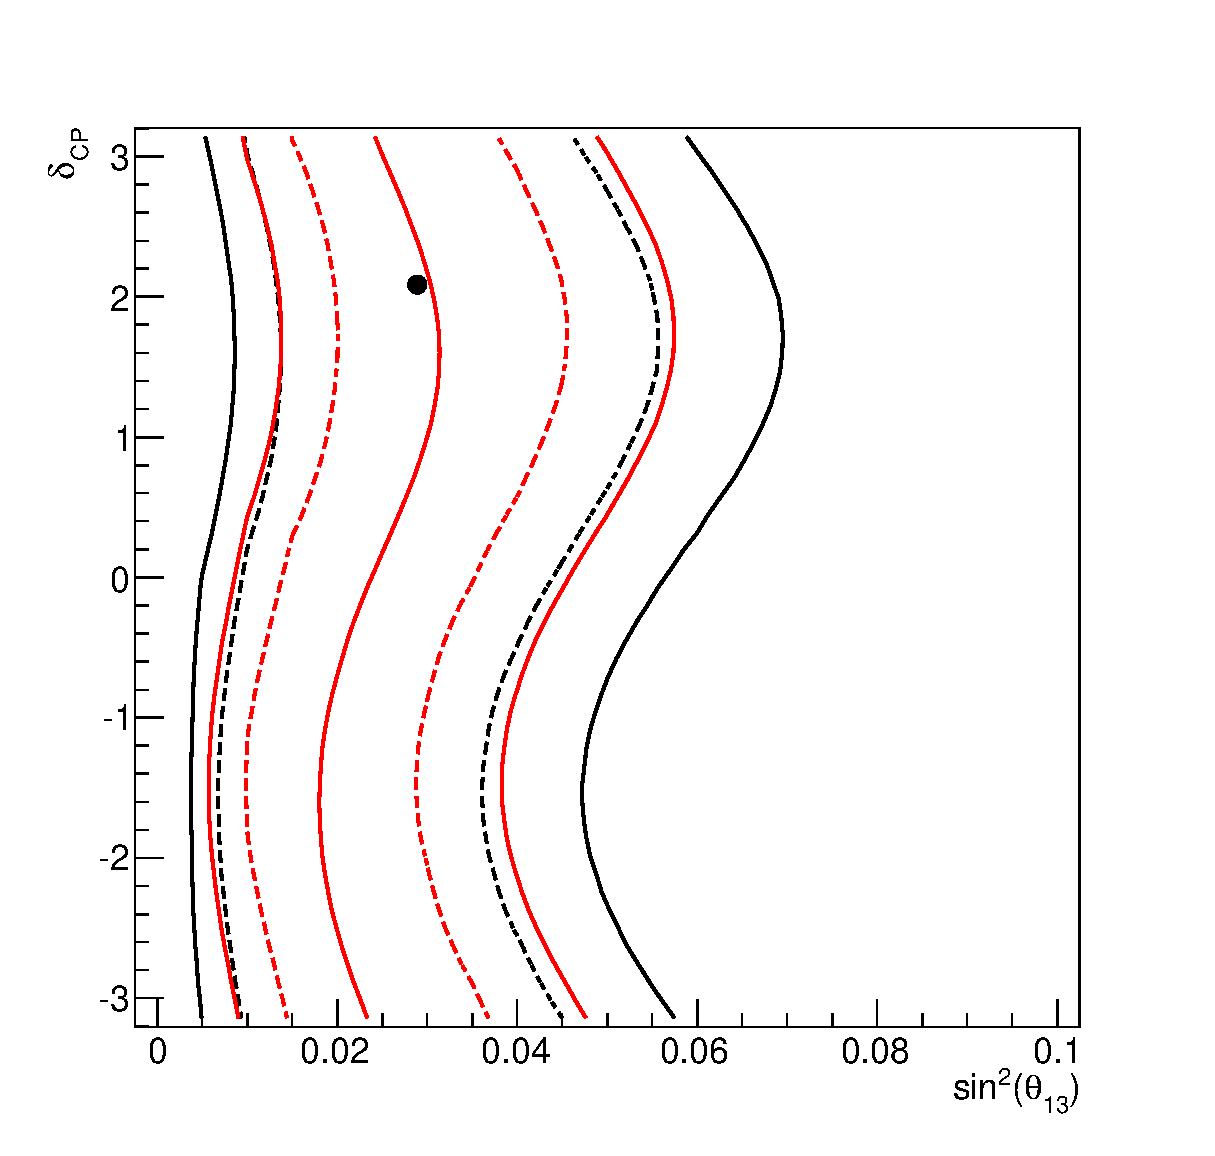
\includegraphics[width=22pc]{./images/results/data_chisq_theta13_deltacp_global_min_new.eps}
\caption {
  68\% (dashed lines) and 90\% (solid lines) CL regions in ($sin^{2}\theta_{13}$, $\delta_{CP}$) space 
  from the analysis of the Run 1+2+3 dataset
   comparing the joint analysis (black) with the stand-alone $\nu_{e}$ appearance (red)
     for Normal Hierarchy. 
  At each point, $\chi^2$ was minimized with respect to
  all oscillation parameters not shown (and not considered to be fixed)
  and all relevant nuisance parameters. Notice that different methods are used to
  construct confidence regions for the joint analysis (global minimum) and for the 
  stand-alone appearance analysis (raster scan). Middle solid red line is the line
  of best-fit points from the raster scan in the stand-alone appearance analysis.
}
\label{fig:run123_confreg_sinsqtheta13_deltacp_nh}
\end{minipage}

\end{figure*}

%...........................................................
%
% contours 
% that can not be compared with stand-alone analyses
% dmsq - sinsqtheta13, sinsqtheta23 - sinsqtheta13
%


\begin{figure*}[htb]

\begin{minipage}[t]{0.98\linewidth}
\center
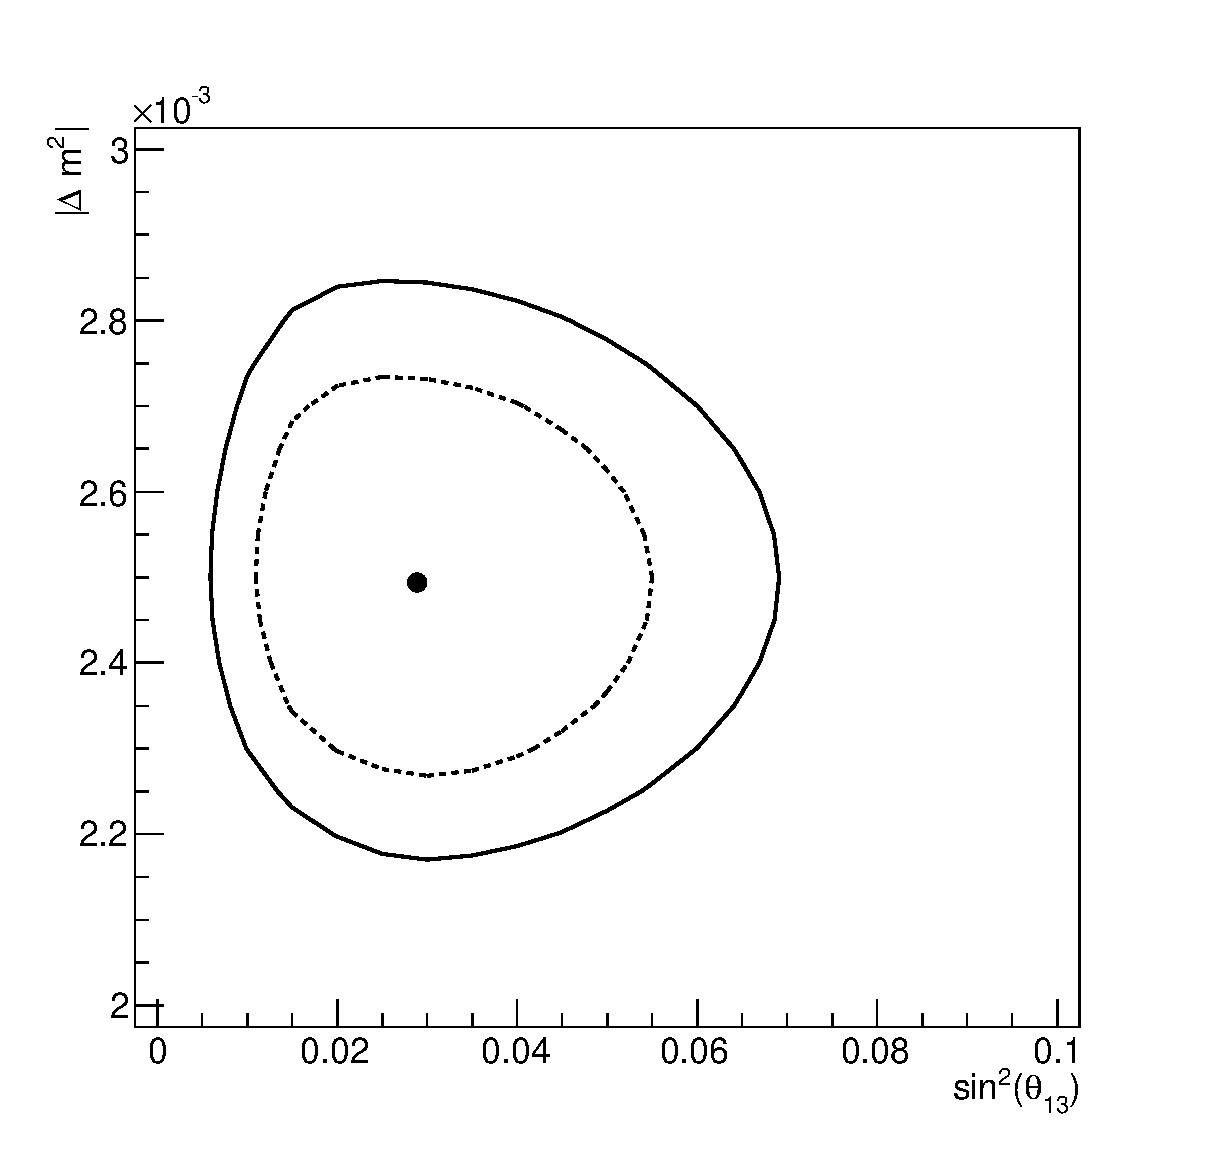
\includegraphics[width=22pc]{./images/results/data_chisq_theta13_dm23sq_global_min_new.eps}
\caption {
  68\% (dashed lines) and 90\% (solid lines) CL regions in ($sin^{2}\theta_{13}$, $|\Delta m^{2}|$) space 
  from the analysis of the Run 1+2+3 dataset  for Normal Hierarchy. 
  At each point, $\chi^2$ was minimized with respect to
  all oscillation parameters not shown (and not considered to be fixed)
  and all relevant nuisance parameters.
}
\label{fig:run123_confreg_sinsqtheta13_Dmsq_nh}
\end{minipage}
\begin{minipage}[t]{0.98\linewidth}
\center
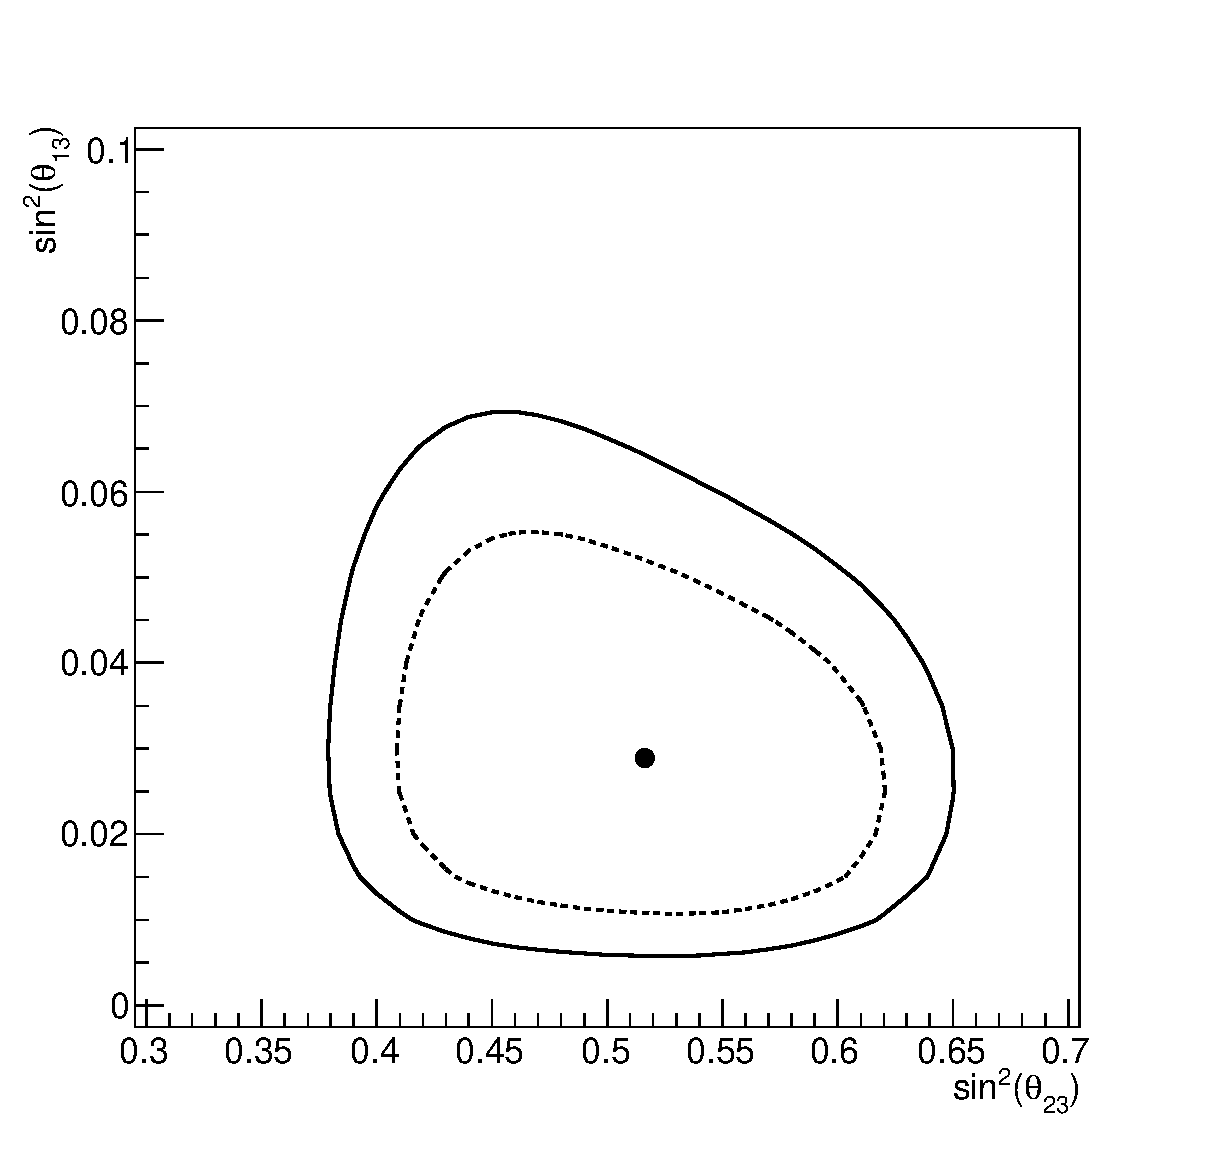
\includegraphics[width=22pc]{./images/results/data_chisq_theta13_theta23_global_min_new.eps}
\caption {
 68\% (dashed lines) and 90\% (solid lines) CL regions in ($sin^{2}\theta_{23}$, $sin^{2}\theta_{13}$) space
  from the analysis of the Run 1+2+3 dataset  for Normal Hierarchy. 
  At each point, $\chi^2$ was minimized with respect to
  all oscillation parameters not shown (and not considered to be fixed)
  and all relevant nuisance parameters.
}
\label{fig:run123_confreg_sinsqtheta23_sinsqtheta13_nh}
\end{minipage}

\end{figure*}


%...........................................................
%
% marginalized (1D) delta\chisq distributions
%

\begin{figure*}[htb]

\begin{minipage}[t]{0.45\linewidth}
\center
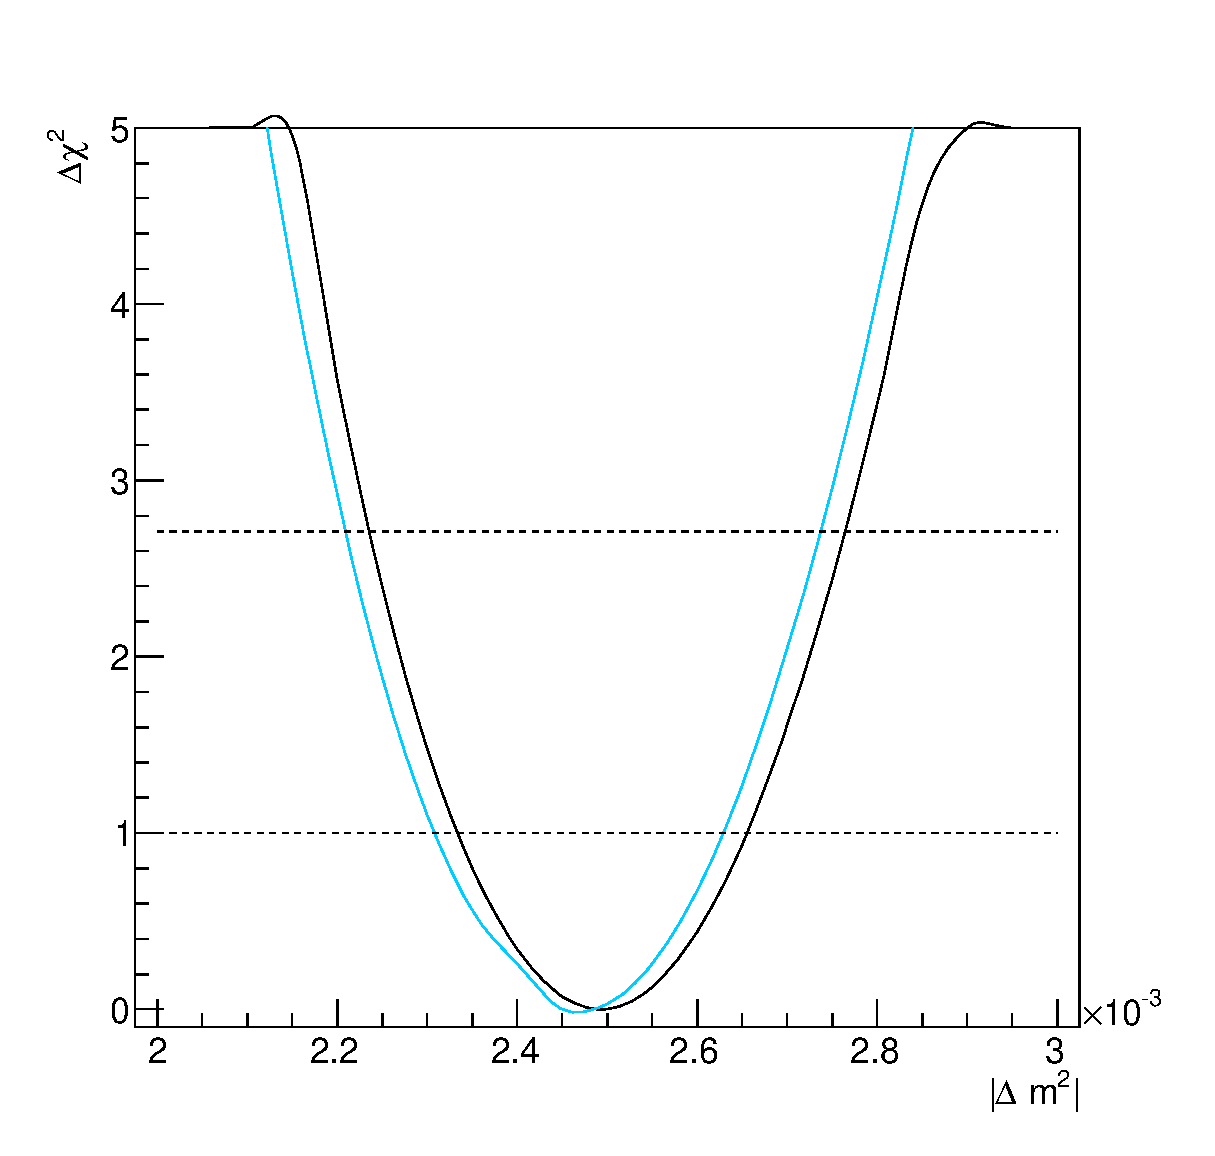
\includegraphics[width=18pc]{./images/results/data_chisq_dm23sq_global_min_mh_new.eps}
\caption {
  $\Delta\chi^2$ as function of $|\Delta m^{2}|$ from the joint 3-flavour oscillation analysis of the Run 1+2+3 dataset.
  Comparing  $\Delta\chi^2$ curves for Normal Hierarchy (black) and Inverted Hierarchy (azure).
  At each point, $\chi^2$ was minimized with respect to
  all oscillation parameters not shown (and not considered to be fixed)
  and all relevant nuisance parameters.
}
\label{fig:run123_dchisq_Dmsq_hcomp}
\end{minipage}
\hspace{0.04\linewidth}
\begin{minipage}[t]{0.45\linewidth}
\center
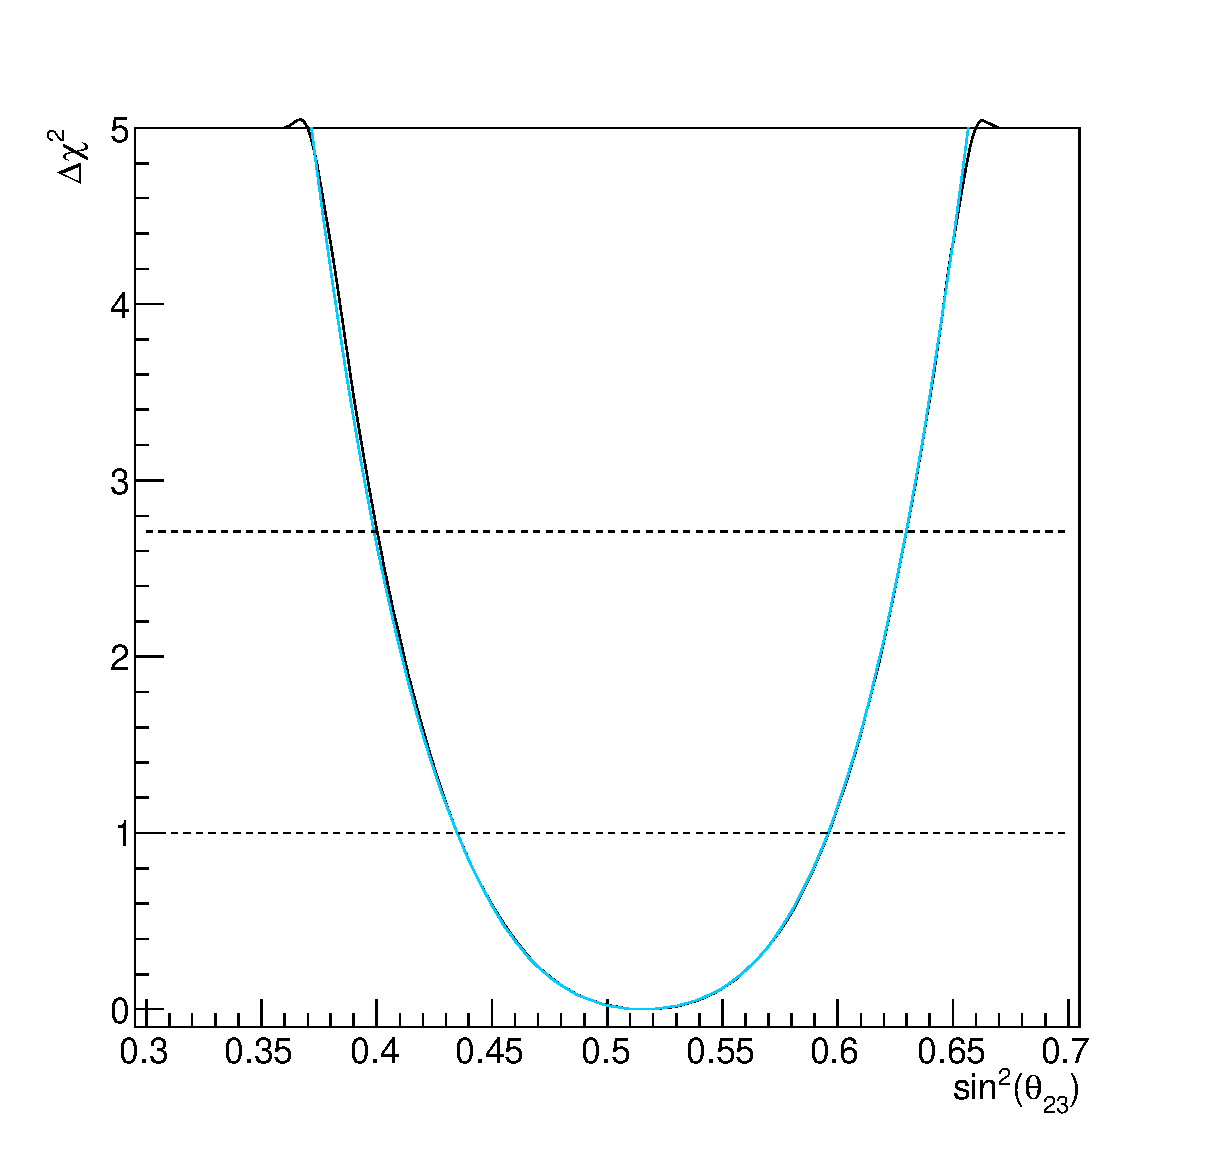
\includegraphics[width=18pc]{./images/results/data_chisq_theta23_global_min_mh_new.eps}
\caption {
  $\Delta\chi^2$ as function of $sin^{2}\theta_{23}$ from the 3-flavour oscillation analysis of the Run 1+2+3 dataset.
  Comparing $\Delta\chi^2$ curves for Normal Hierarchy (black) and Inverted Hierarchy (azure).	
  At each point, $\chi^2$ was minimized with respect to
  all oscillation parameters not shown (and not considered to be fixed)
  and all relevant nuisance parameters.
}
\label{fig:run123_dchisq_sinsqtheta23_hcomp}
\end{minipage}

\vfill
\vspace*{0.7cm}

\begin{minipage}[t]{0.45\linewidth}
\center
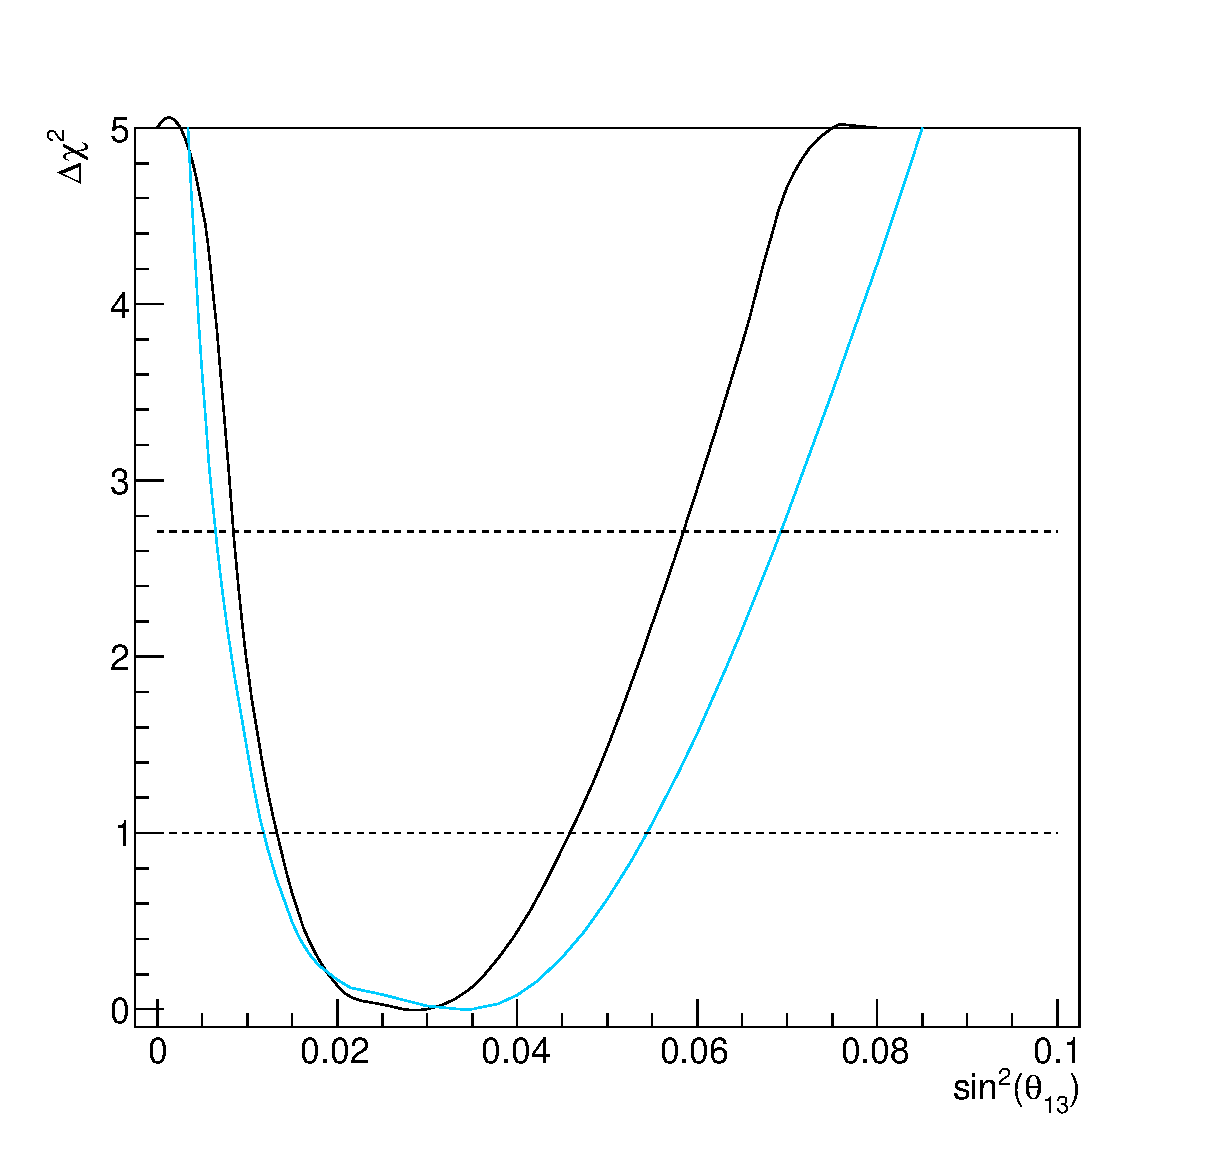
\includegraphics[width=18pc]{./images/results/data_chisq_theta13_global_min_mh_new.eps}
\caption {
  $\Delta\chi^2$ as function of $sin^{2}\theta_{13}$ from the 3-flavour oscillation analysis of the Run 1+2+3 dataset.
  Comparing $\Delta\chi^2$ curves for Normal Hierarchy (black) and Inverted Hierarchy (azure).
  At each point, $\chi^2$ was minimized with respect to
  all oscillation parameters not shown (and not considered to be fixed)
  and all relevant nuisance parameters.
}
\label{fig:run123_dchisq_sinsqtheta13_hcomp}
\end{minipage}
\hspace{0.04\linewidth}
\begin{minipage}[t]{0.45\linewidth}
\center
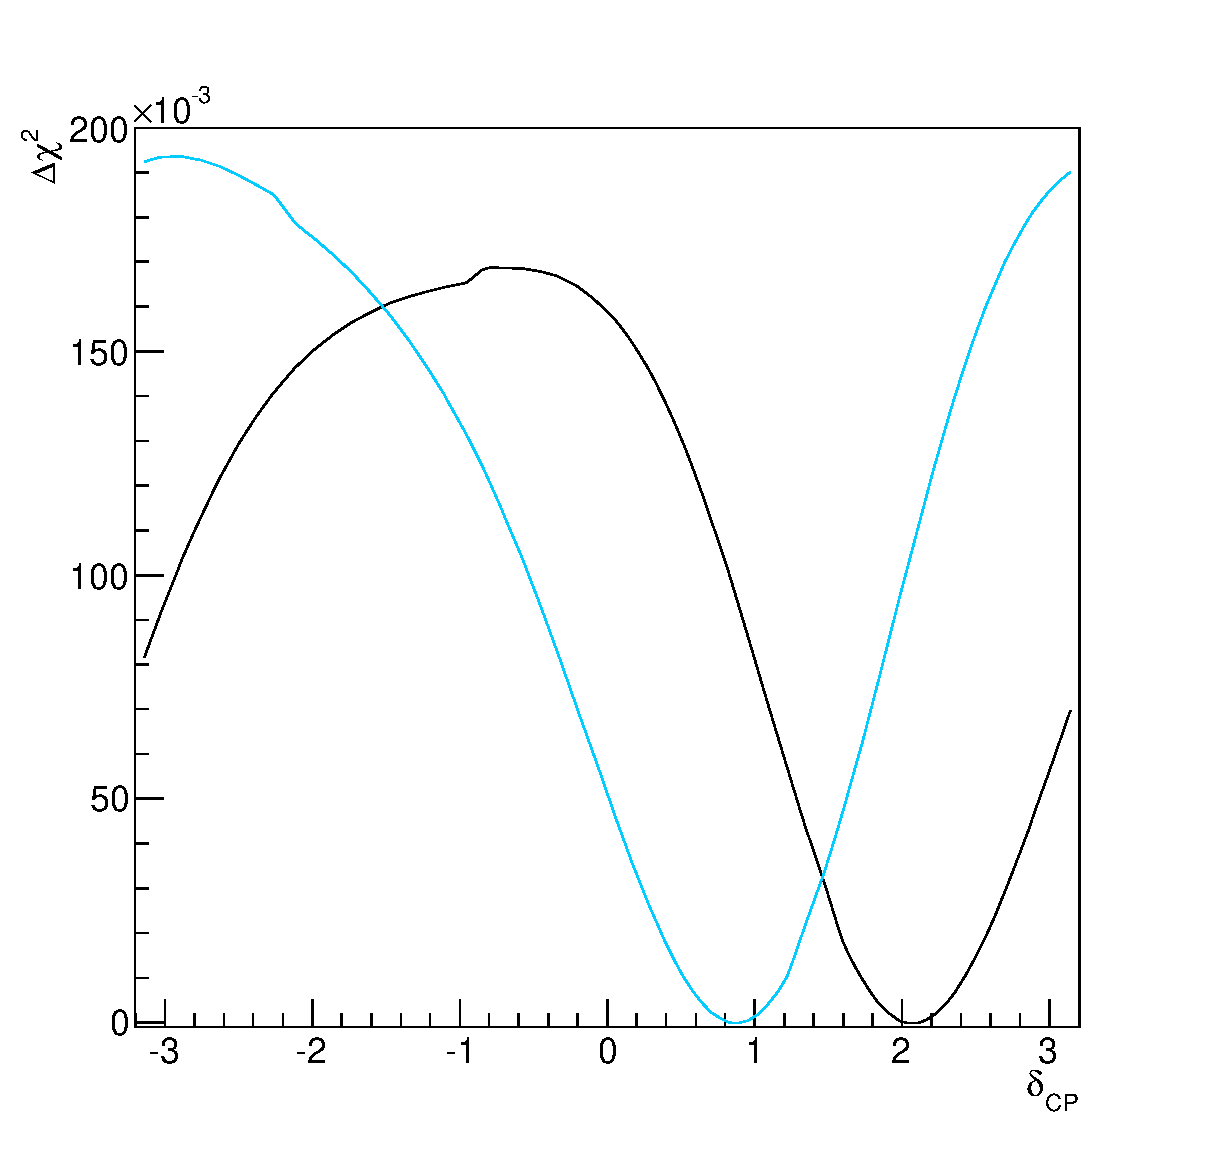
\includegraphics[width=18pc]{./images/results/data_chisq_deltacp_global_min_mh_new.eps}
\caption {
  $\Delta\chi^2$ as function of $\delta_{CP}$ from the 3-flavour oscillation analysis of the Run 1+2+3 dataset.
  Comparing $\Delta\chi^2$ curves for Normal Hierarchy (black) with Inverted Hierarchy (azure).
  At each point, $\chi^2$ was minimized with respect to
  all oscillation parameters not shown (and not considered to be fixed)
  and all relevant nuisance parameters.
}
\label{fig:run123_dchisq_deltacp_hcomp}
\end{minipage}

\end{figure*}

%...........................................................
%
% contours 
% that can be compared with stand-alone analyses
% dmsq - sinsqtheta23, deltacp - sinsqtheta13
%

\begin{figure*}[htb]

\begin{minipage}[t]{0.98\linewidth}
\center
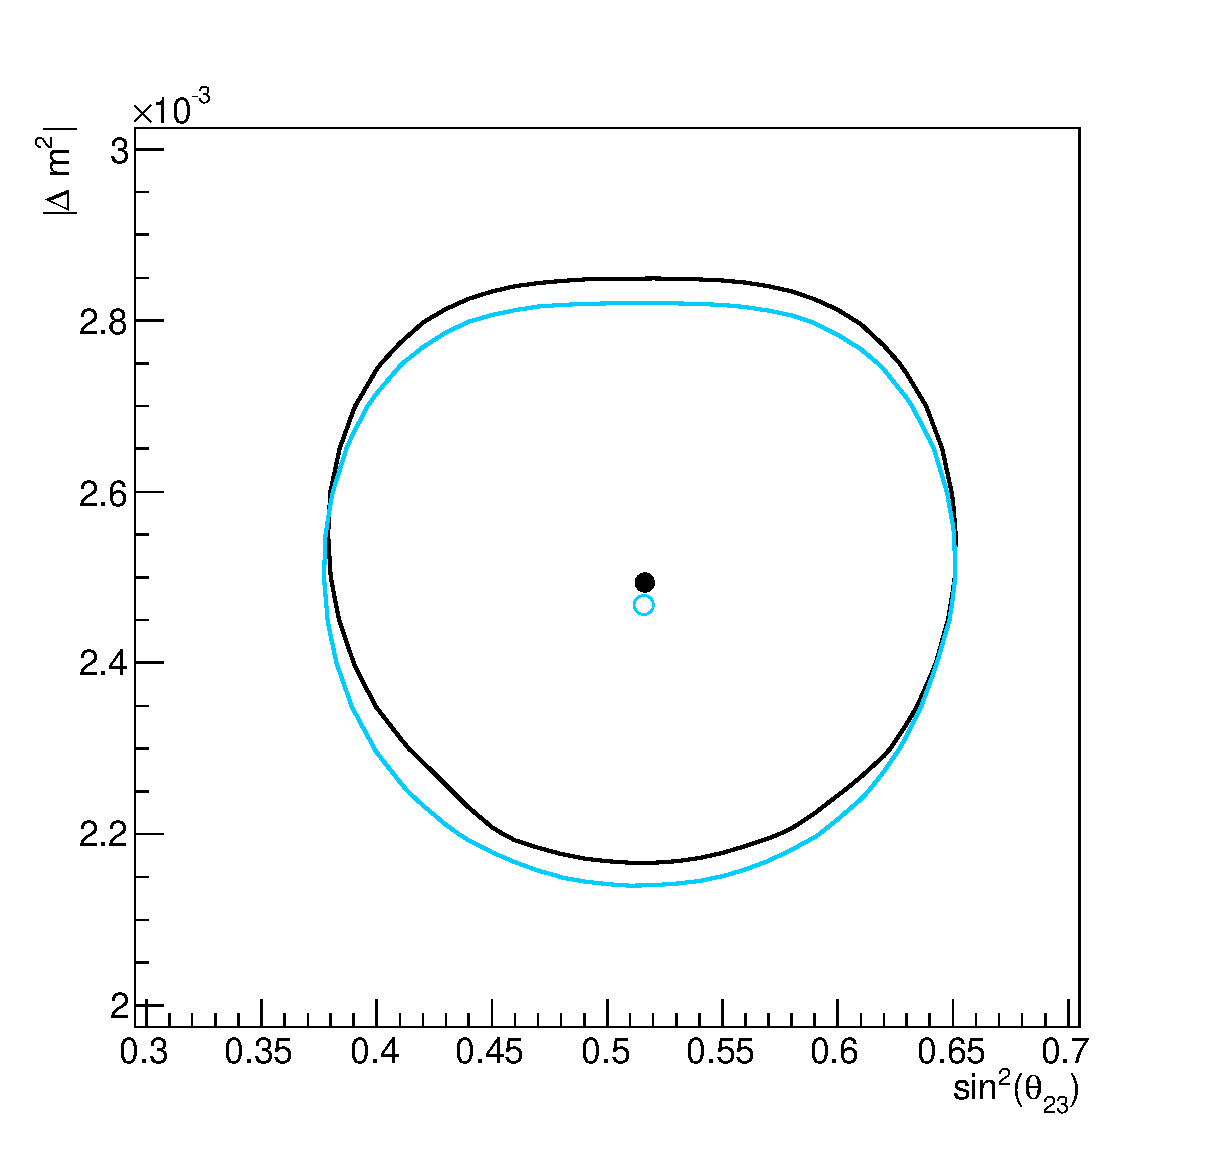
\includegraphics[width=20pc]{./images/results/data_chisq_theta23_dm23sq_global_min_mh_new.eps}
\caption {
  90\% CL regions in ($sin^{2}\theta_{23}$, $|\Delta m^{2}|$) space 
  from the joint 3-flavour oscillation analysis of the Run 1+2+3 dataset,
  comparing contours for the Normal Hierarchy (black) and Inverted Hierarchy (azure).	
  At each point, $\chi^2$ was minimized with respect to
  all oscillation parameters not shown (and not considered to be fixed)
  and all relevant nuisance parameters.
}
\label{fig:run123_confreg_sinsqtheta23_Dmsq_hcomp}
\end{minipage}
\begin{minipage}[t]{0.98\linewidth}
\center
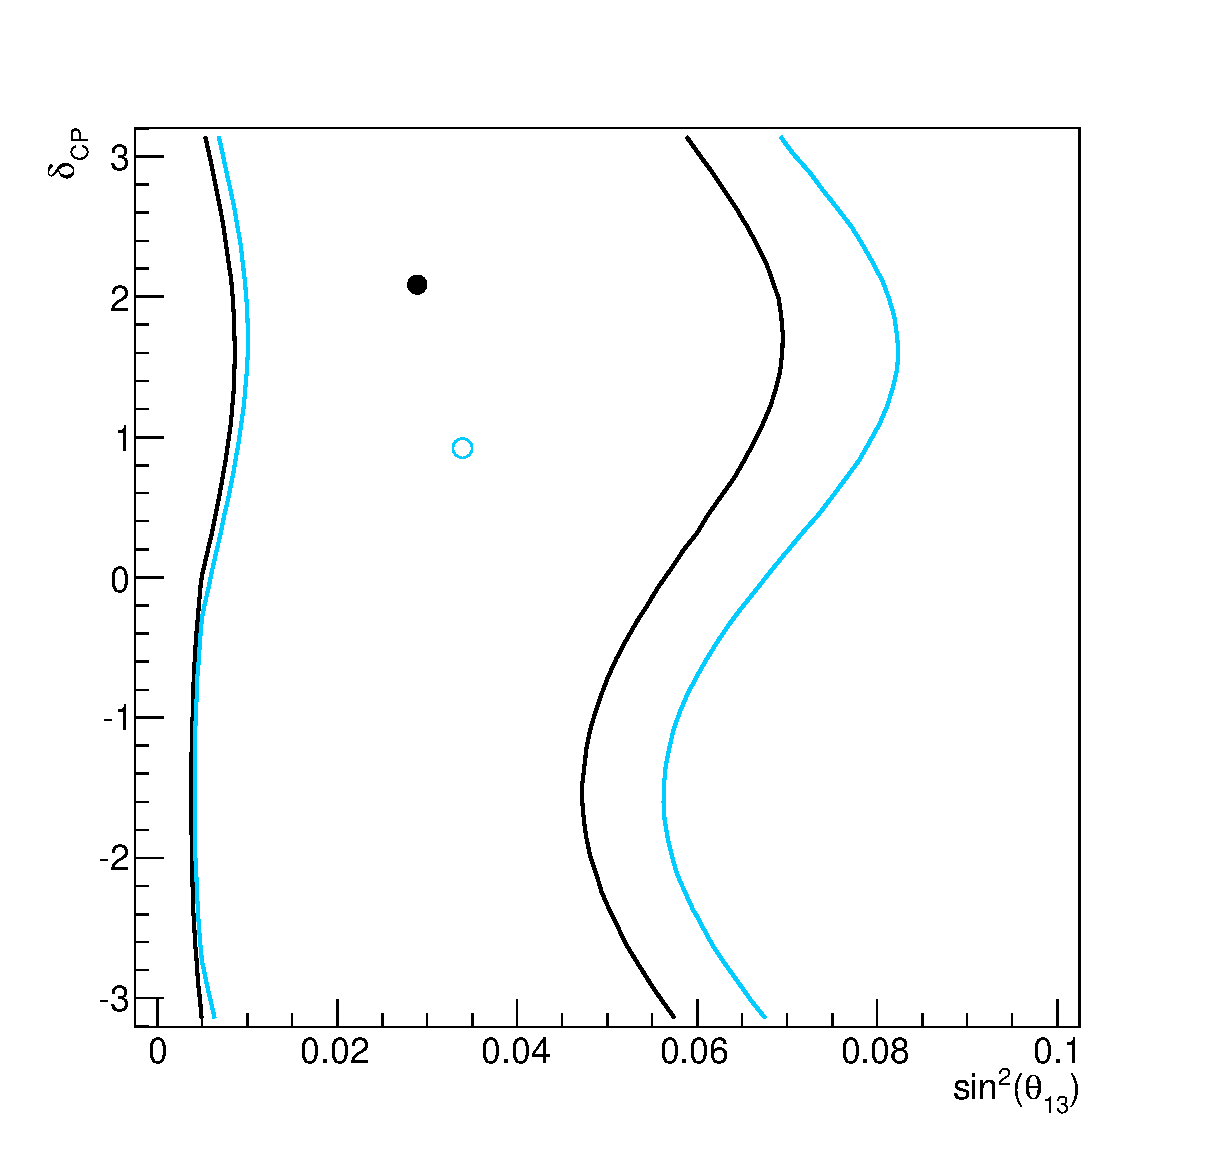
\includegraphics[width=20pc]{./images/results/data_chisq_theta13_deltacp_global_min_mh_new.eps}
\caption {
  90\% CL regions in ($sin^{2}\theta_{13}$, $\delta_{CP}$) space 
  from the joint 3-flavour oscillation analysis of the Run 1+2+3 dataset,
  comparing contours for the Normal Hierarchy (black) and Inverted Hierarchy (azure).
  At each point, $\chi^2$ was minimized with respect to
  all oscillation parameters not shown (and not considered to be fixed)
  and all relevant nuisance parameters.
}
\label{fig:run123_confreg_sinsqtheta13_deltacp_hcomp}
\end{minipage}

\end{figure*}

%...........................................................
%
% contours 
% that can not be compared with stand-alone analyses
% dmsq - sinsqtheta13, sinsqtheta23 - sinsqtheta13
%


\begin{figure*}[htb]

\begin{minipage}[t]{0.98\linewidth}
\center
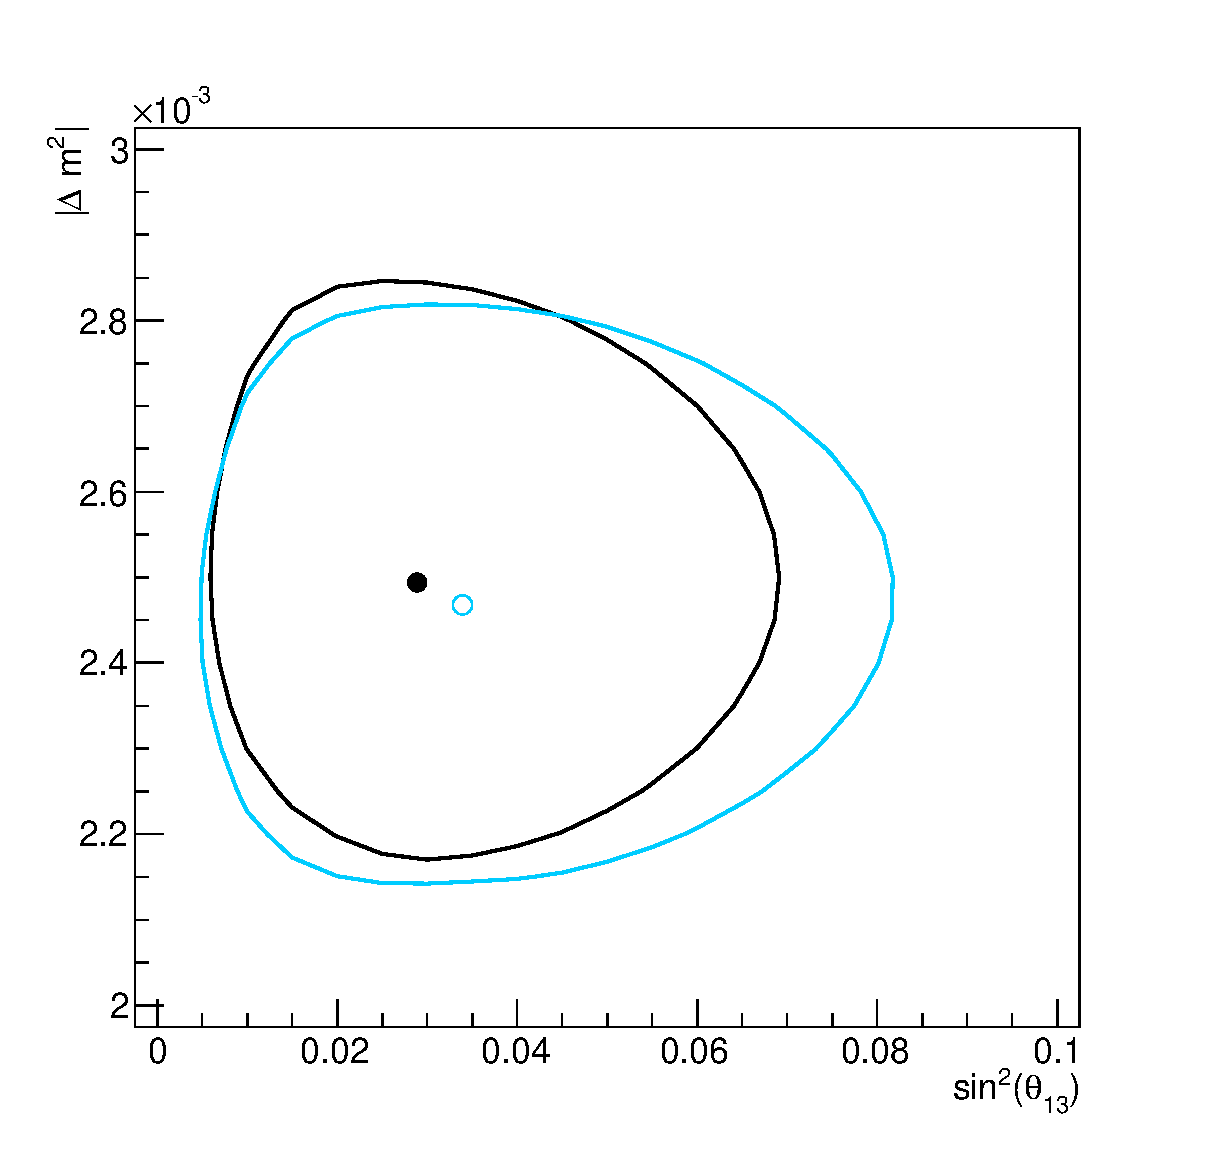
\includegraphics[width=22pc]{./images/results/data_chisq_theta13_dm23sq_global_min_mh_new.eps}
\caption {
90\% CL regions in ($sin^{2}\theta_{13}$, $|\Delta m^{2}|$) space 
  from the joint 3-flavour oscillation analysis of the Run 1+2+3 dataset,
  comparing contours for the Normal Hierarchy (black) and Inverted Hierarchy (azure).
  At each point, $\chi^2$ was minimized with respect to
  all oscillation parameters not shown (and not considered to be fixed)
  and all relevant nuisance parameters.
}
\label{fig:run123_confreg_sinsqtheta13_Dmsq_hcomp}
\end{minipage}
\begin{minipage}[t]{0.98\linewidth}
\center
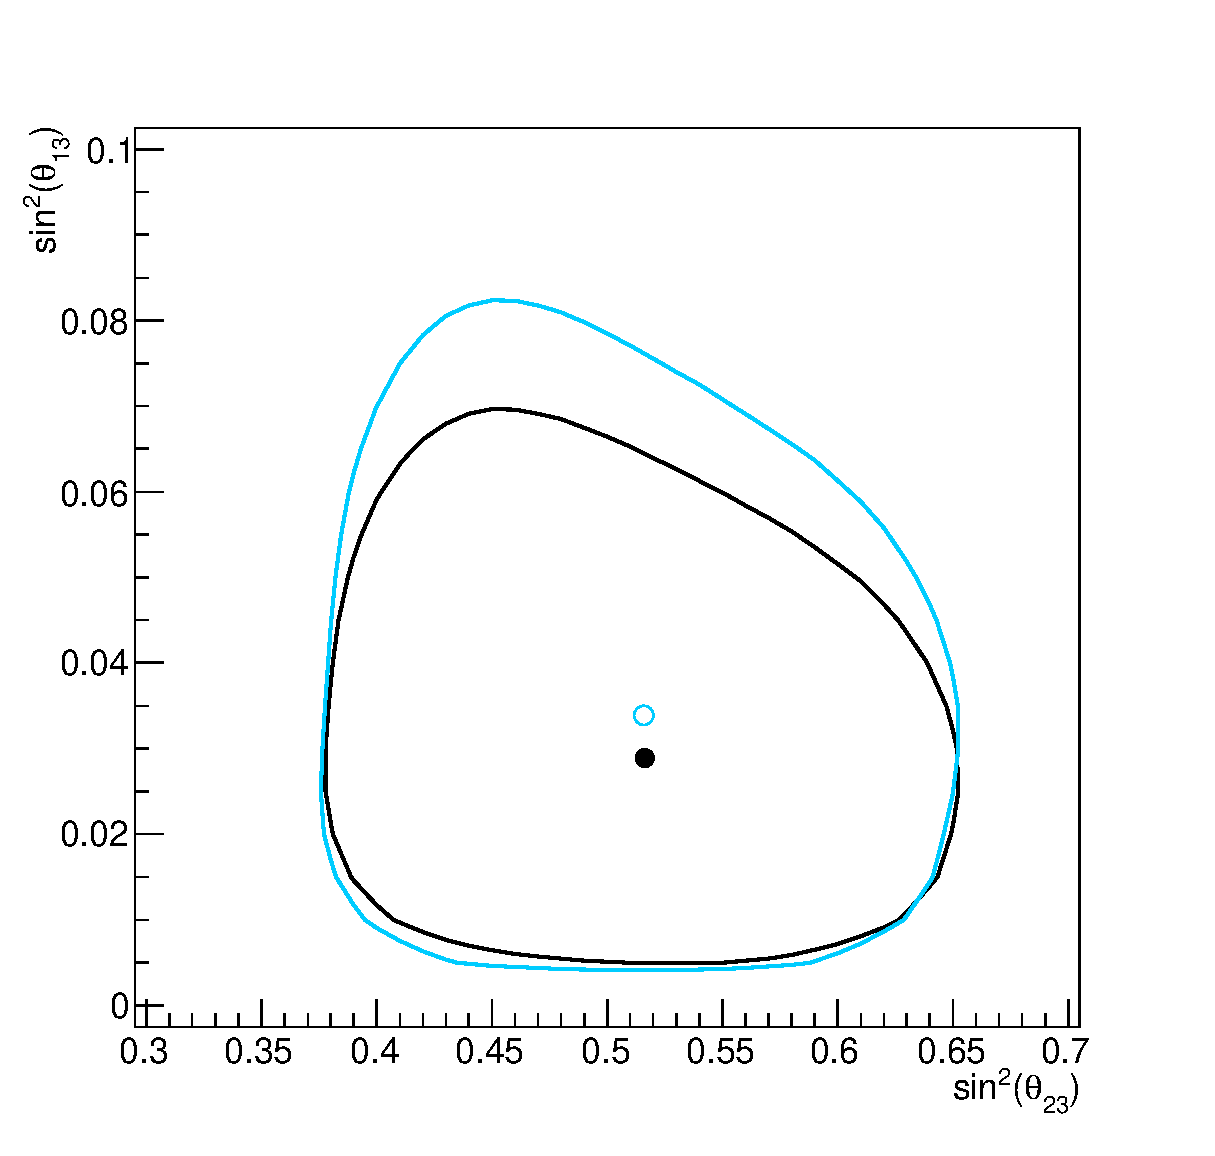
\includegraphics[width=22pc]{./images/results/data_chisq_theta13_theta23_global_min_mh_new.eps}
\caption {
  90\% CL regions in ($sin^{2}\theta_{23}$, $sin^{2}\theta_{13}$) space
  from the joint 3-flavour oscillation analysis of the Run 1+2+3 dataset,
  comparing contours for the Normal Hierarchy (black) and Inverted Hierarchy (azure).
  At each point, $\chi^2$ was minimized with respect to
  all oscillation parameters not shown (and not considered to be fixed)
  and all relevant nuisance parameters.
}
\label{fig:run123_confreg_sinsqtheta23_sinsqtheta13_hcomp}
\end{minipage}

\end{figure*}


%...........................................................
%
% m2D theta13-deltacp contours with raster scan also for joint
%

\clearpage

\begin{figure*}[htb]

\begin{minipage}[t]{0.98\linewidth}
\center
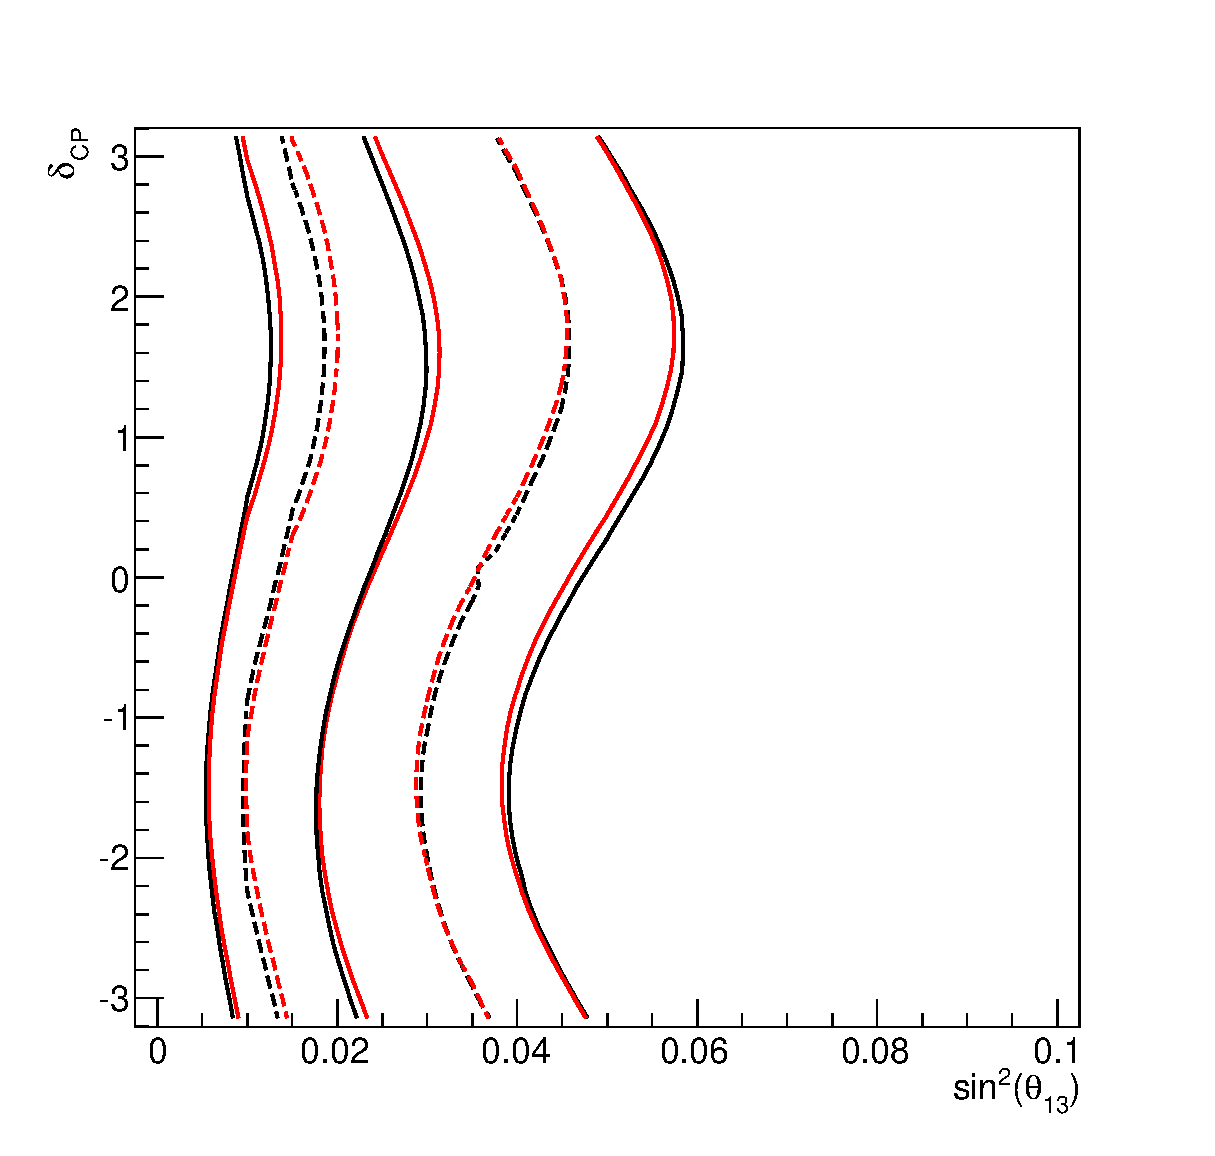
\includegraphics[width=22pc]{./images/results/data_nh_chisq_theta13_deltacp_raster.eps}
\caption {
  68\% (dashed lines) and 90\% (solid lines) CL regions in ($sin^{2}\theta_{13}$, $\delta_{CP}$) space 
  from the analysis of the Run 1+2+3 dataset
   comparing the joint analysis (black) with the stand-alone $\nu_{e}$ appearance (red)
     for Normal Hierarchy, using the raster scan in both analyses. Middle solid black (red) line is the line
  of best-fit points from the raster scan in the joint (stand-alone appearance) analysis.
 }
\label{fig:run123_confreg_sinsqtheta13_deltacp_raster_nh}
\end{minipage}
\begin{minipage}[t]{0.98\linewidth}
\center
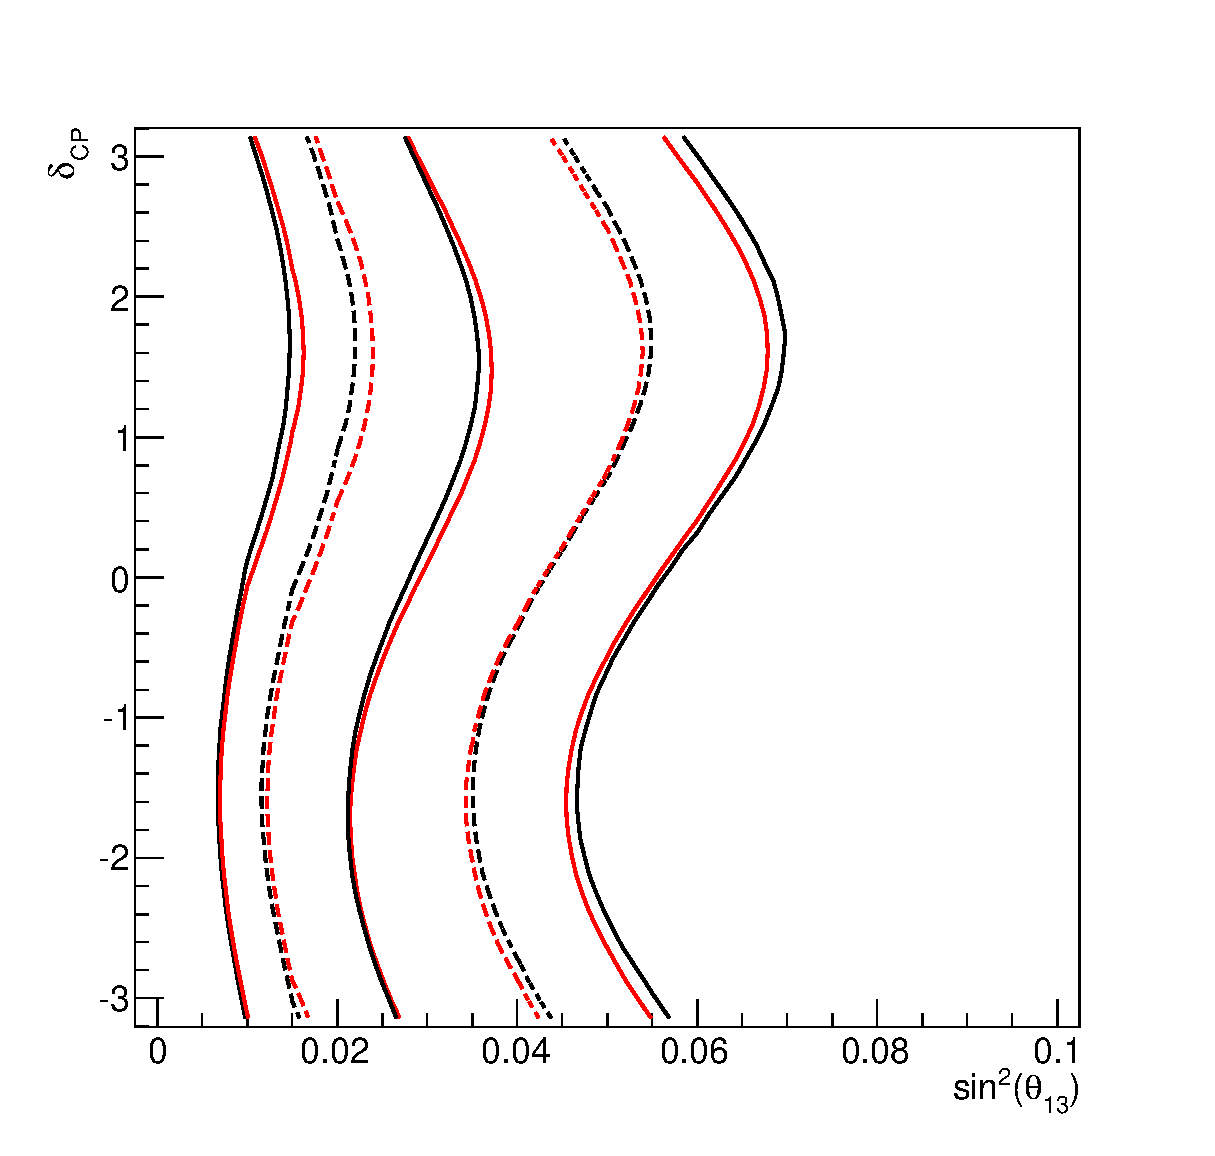
\includegraphics[width=22pc]{./images/results/data_ih_chisq_theta13_deltacp_raster.eps}
\caption {
  68\% (dashed lines) and 90\% (solid lines) CL regions in ($sin^{2}\theta_{13}$, $\delta_{CP}$) space 
  from the analysis of the Run 1+2+3 dataset
    comparing the joint analysis (black) with the stand-alone $\nu_{e}$ appearance (red)
     for Inverted Hierarchy, using the raster scan in both analyses. Middle solid black (red) line is the line
  of best-fit points from the raster scan in the joint (stand-alone appearance) analysis.
     }
\label{fig:run123_confreg_sinsqtheta13_deltacp_raster_ih}
\end{minipage}

\end{figure*}


\clearpage

%...........................................................
%
% marginalized (1D) delta\chisq distributions
%

%\begin{figure*}[htb]

%\begin{minipage}[t]{0.45\linewidth}
%\center
%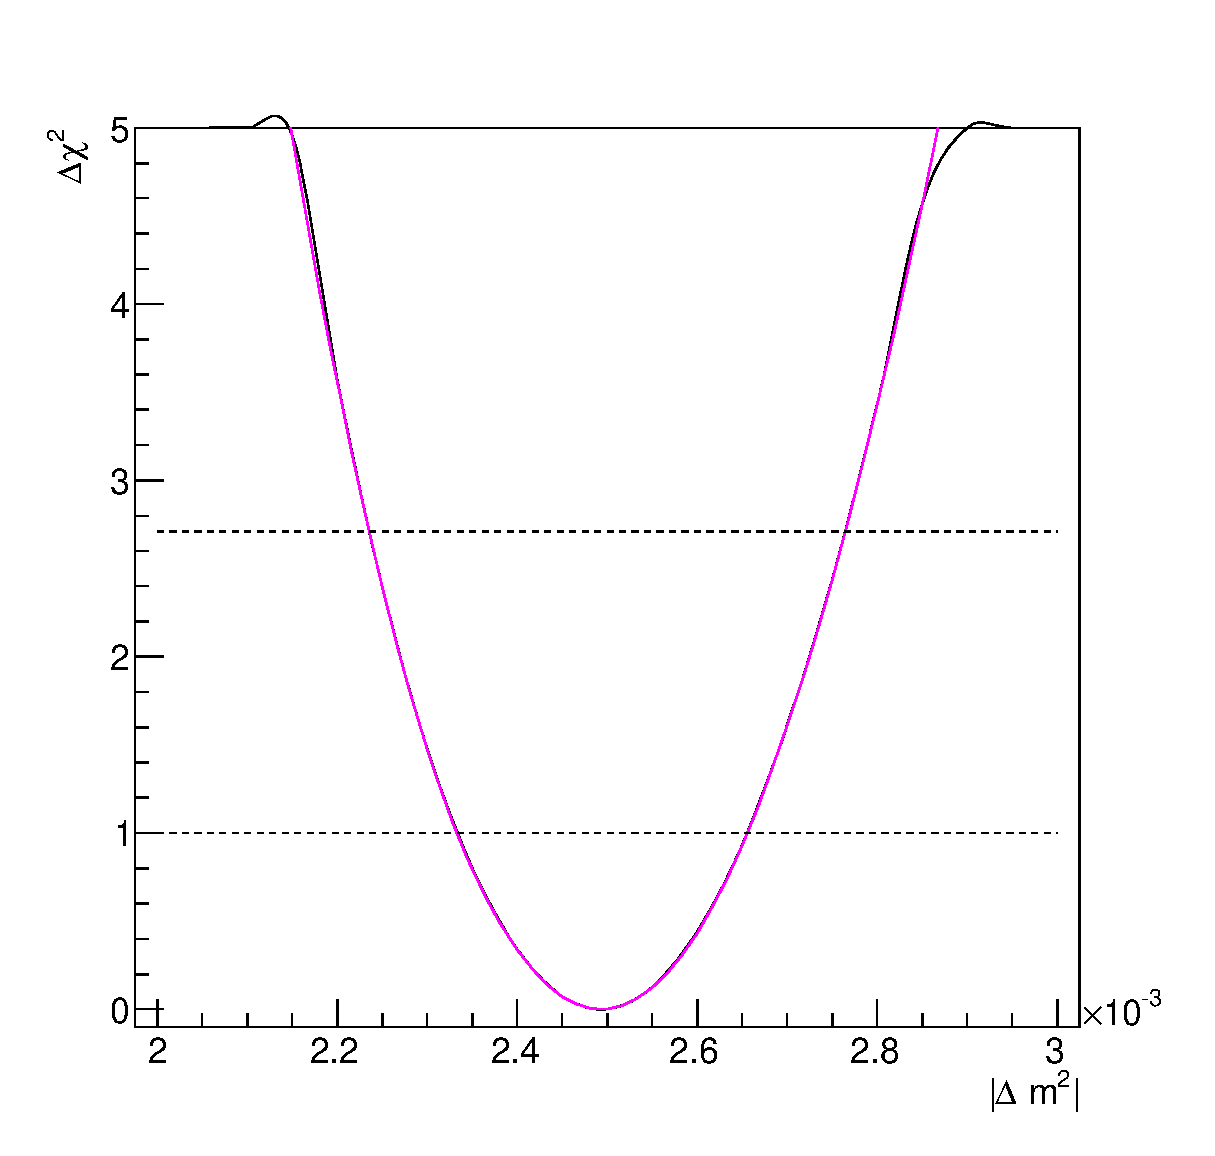
\includegraphics[width=18pc]{./images/results/data_chisq_dm23sq_global_min_2nd.eps}
%\caption {
  %$\Delta\chi^2$ as function of $|\Delta m^{2}|$ from the joint 3-flavour oscillation analysis of the Run 1+2+3 dataset.
 % Comparing $\Delta\chi^2$ curves for Normal Hierarchy with initial value in 1st octant (black) and 2nd octant (magenta).
 % At each point, $\chi^2$ was minimized with respect to
 % all oscillation parameters not shown (and not considered to be fixed)
 % and all relevant nuisance parameters.
%}
%\label{fig:run123_dchisq_Dmsq_octcomp}
%\end{minipage}

%\vfill
%\vspace*{0.7cm}

%\begin{minipage}[t]{0.45\linewidth}
%\center
%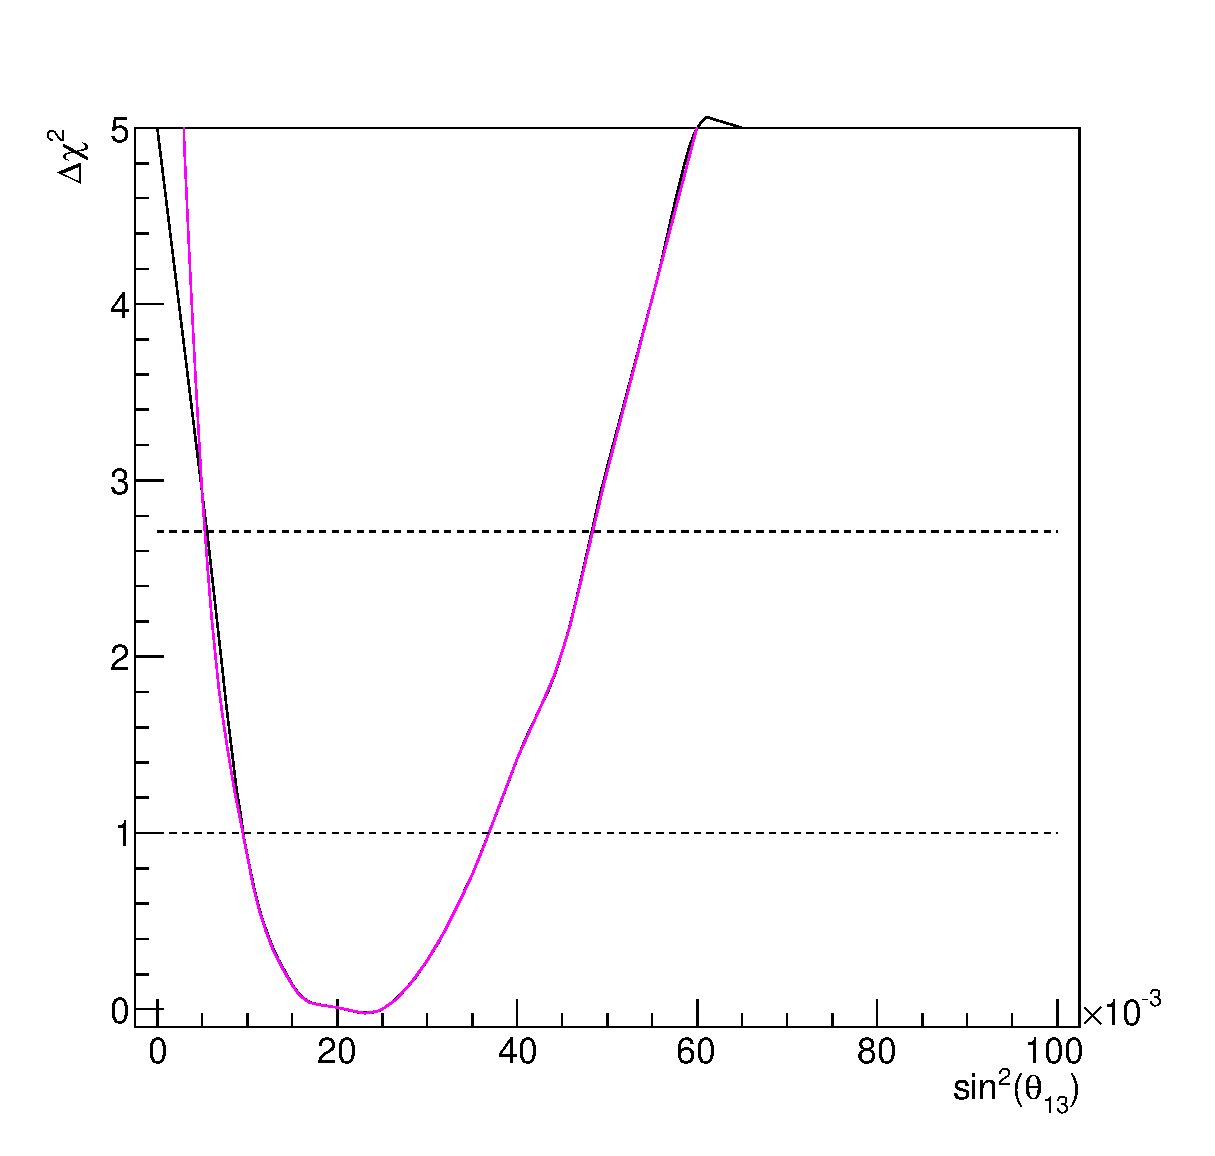
\includegraphics[width=18pc]{./images/results/data_chisq_theta13_global_min_2nd.eps}
%\caption {
 % $\Delta\chi^2$ as function of $sin^{2}\theta_{13}$ from the joint 3-flavour oscillation analysis of the Run 1+2+3 dataset.
 % Comparing $\Delta\chi^2$ curves for Normal Hierarchy with initial value in 1st octant (black) and 2nd octant (magenta).
 % At each point, $\chi^2$ was minimized with respect to
 % all oscillation parameters not shown (and not considered to be fixed)
 % and all relevant nuisance parameters.
%}
%\label{fig:run123_dchisq_sinsqtheta13_octcomp}
%\end{minipage}
%\hspace{0.04\linewidth}
%\begin{minipage}[t]{0.45\linewidth}
%\center
%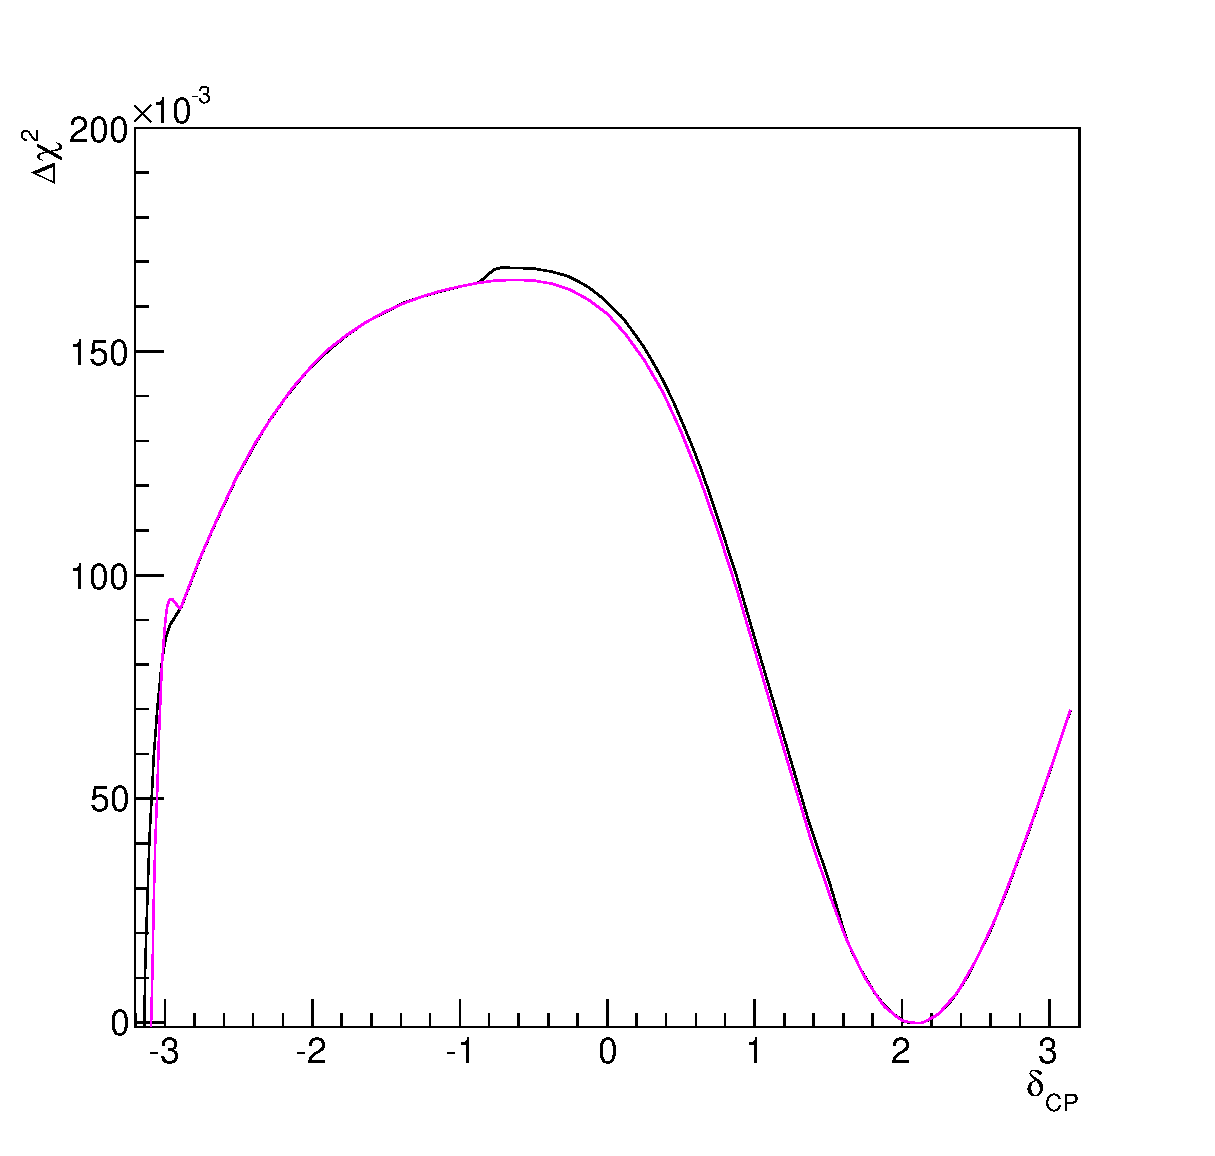
\includegraphics[width=18pc]{./images/results/data_chisq_deltacp_global_min_2nd.eps}
%\caption {
  %$\Delta\chi^2$ as function of $\delta_{CP}$ from the joint 3-flavour oscillation analysis of the Run 1+2+3 dataset.
  %Comparing $\Delta\chi^2$ curves for Normal Hierarchy with initial value in 1st octant (black) and 2nd octant (magenta).
  %At each point, $\chi^2$ was minimized with respect to
  %all oscillation parameters not shown (and not considered to be fixed)
  %and all relevant nuisance parameters.
%}
%\label{fig:run123_dchisq_deltacp_octcomp}
%\end{minipage}

%\end{figure*}


%...........................................................
%
% contours 
% that can not be compared with stand-alone analyses
% dmsq - sinsqtheta13, sinsqtheta23 - sinsqtheta13
%


%\begin{figure*}[htb]
%\begin{minipage}[t]{0.98\linewidth}
%\center
%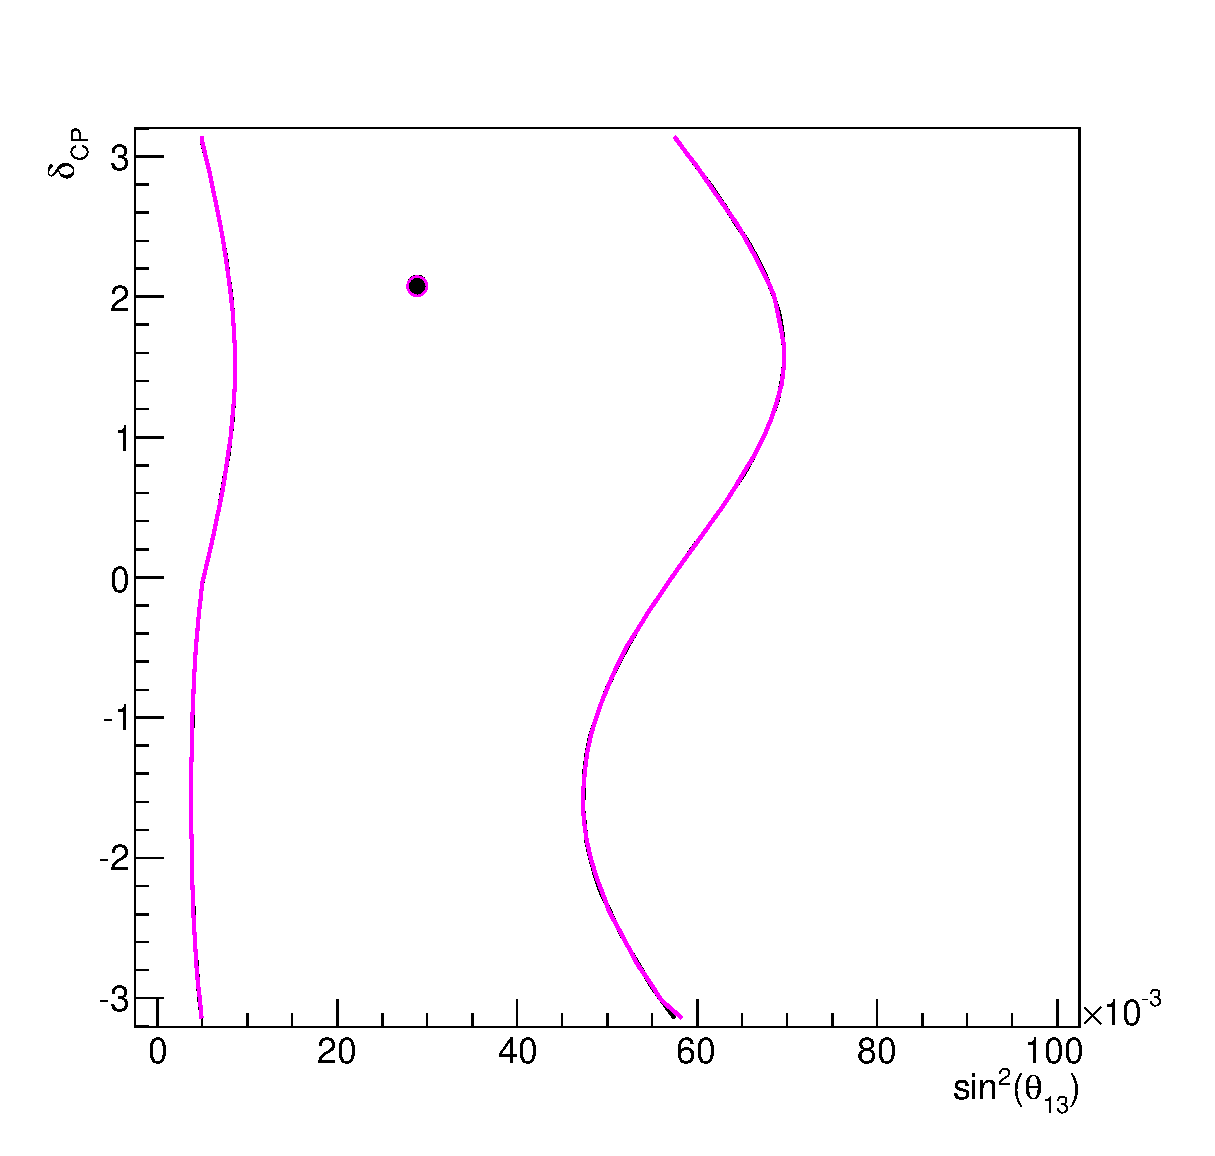
\includegraphics[width=22pc]{./images/results/data_chisq_theta13_deltacp_global_min_2nd.eps}
%\caption {
 % 68\% and 90\% CL regions in ($sin^{2}\theta_{13}$, $\delta_{CP}$) space 
  %from the joint 3-flavour oscillation analysis of the Run 1+2+3 dataset.
 % Comparing contours for Normal Hierarchy with initial value in 1st octant (black) and 2nd octant (magenta).
 % At each point, $\chi^2$ was minimized with respect to
 % all oscillation parameters not shown (and not considered to be fixed)
 % and all relevant nuisance parameters.
%}
%\label{fig:run123_confreg_sinsqtheta13_deltacp_octcomp}
%\end{minipage}
%\begin{minipage}[t]{0.98\linewidth}
%\center
%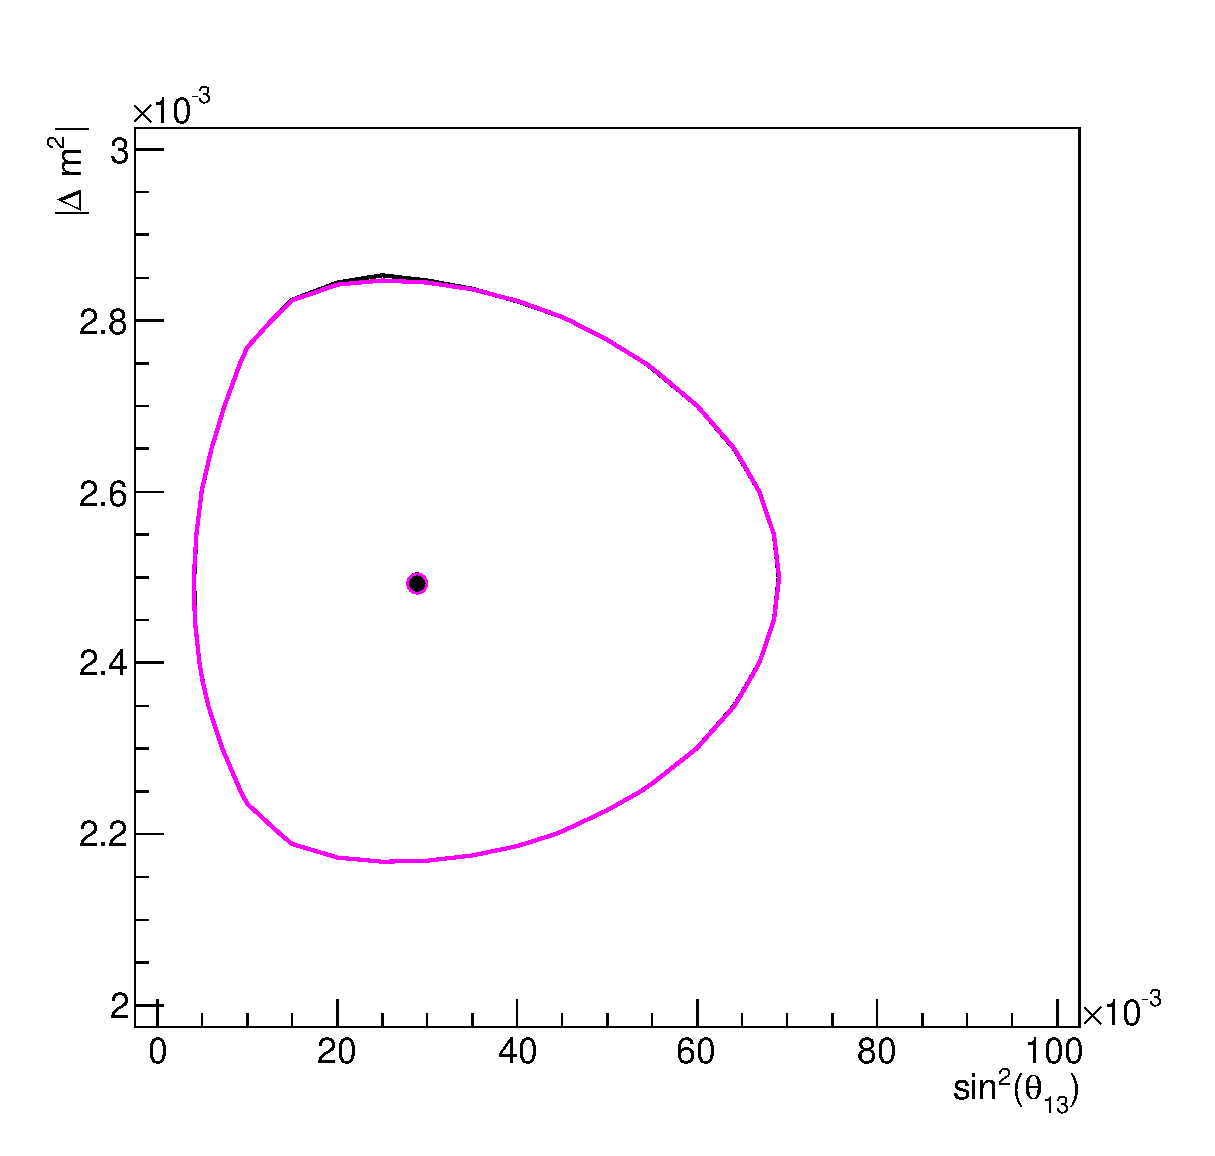
\includegraphics[width=22pc]{./images/results/data_chisq_theta13_dm23sq_global_min_2nd.eps}
%\caption {
 % 68\% and 90\% CL regions in ($sin^{2}\theta_{13}$, $|\Delta m^{2}|$) space 
  %from the joint 3-flavour oscillation analysis of the Run 1+2+3 dataset.
 % Comparing contours for Normal Hierarchy with initial value in 1st octant (black) and 2nd octant (magenta).
 % At each point, $\chi^2$ was minimized with respect to
 % all oscillation parameters not shown (and not considered to be fixed)
 % and all relevant nuisance parameters.
%}
%\label{fig:run123_confreg_sinsqtheta13_Dmsq_octcomp}
%\end{minipage}
%\end{figure*}





